%-----------------------------------------------------------------------------%
\addcontentsline{toc}{chapter}{LAMPIRAN 1}
\chapter*{Lampiran 1}
\newappendix{Lampiran 1. User Persona}
\begin{figure}[H]
	\center
	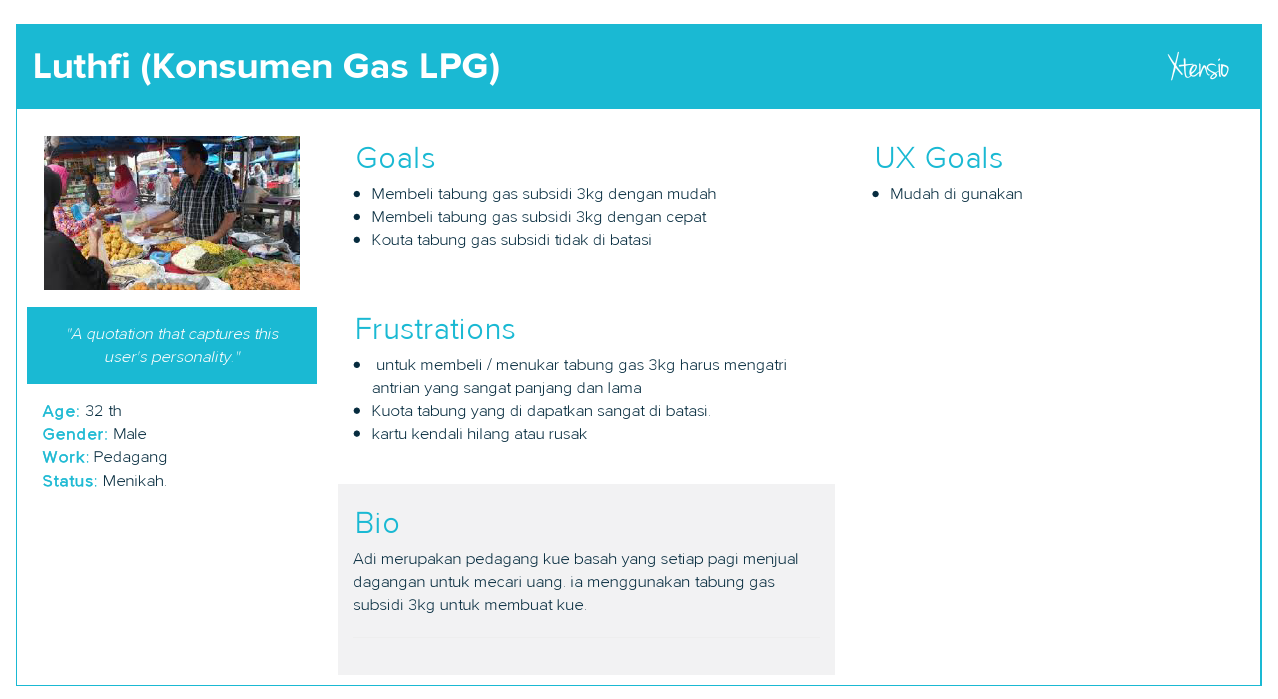
\includegraphics [width = 15cm]{gambar/persona/konsumen}
\end{figure}

\begin{figure}[H]
	\center
	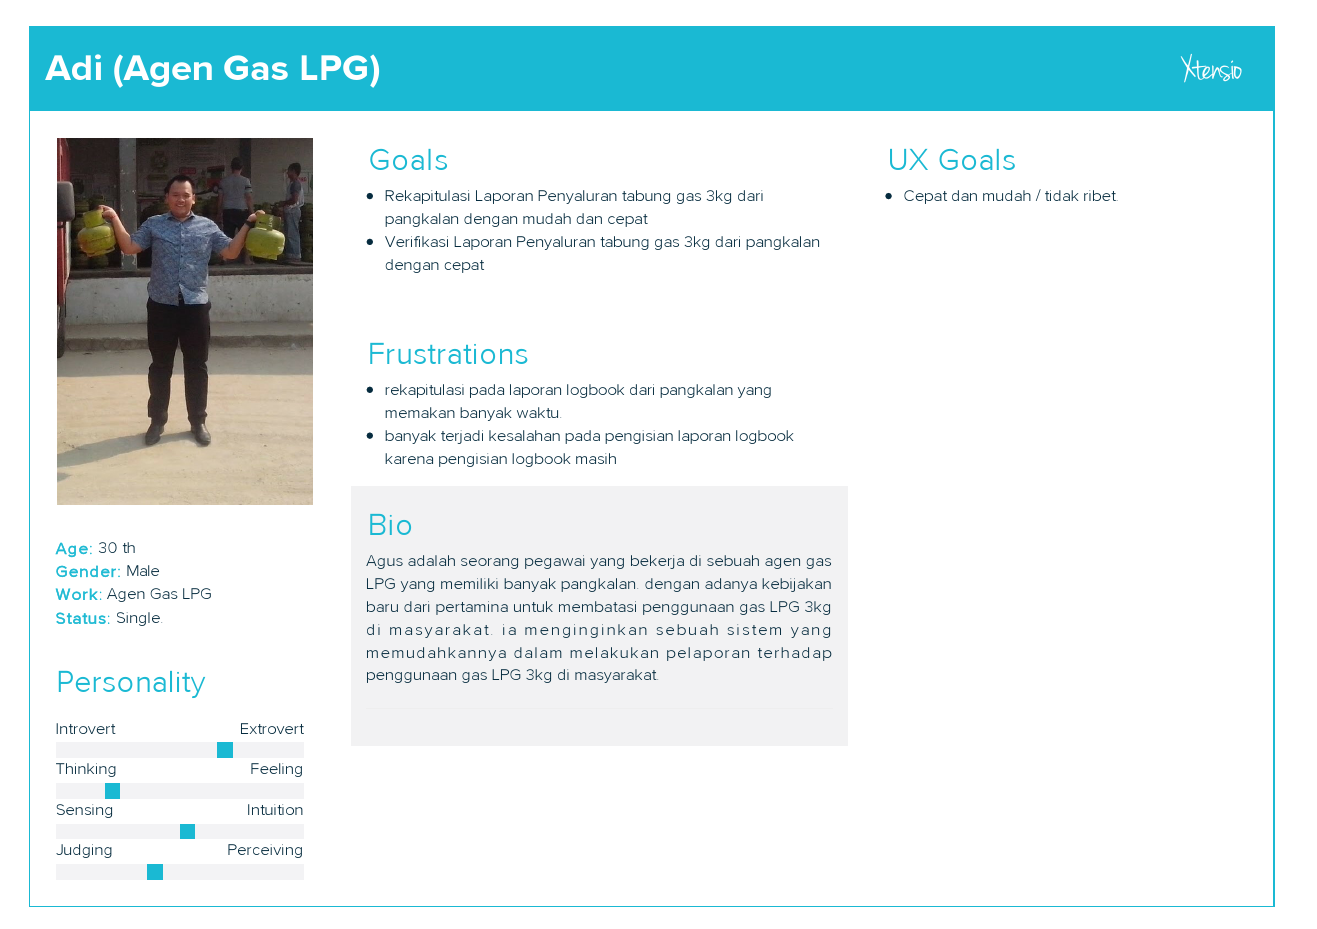
\includegraphics [width = 15cm]{gambar/persona/agen}
\end{figure}

\begin{figure}[H]
	\center
	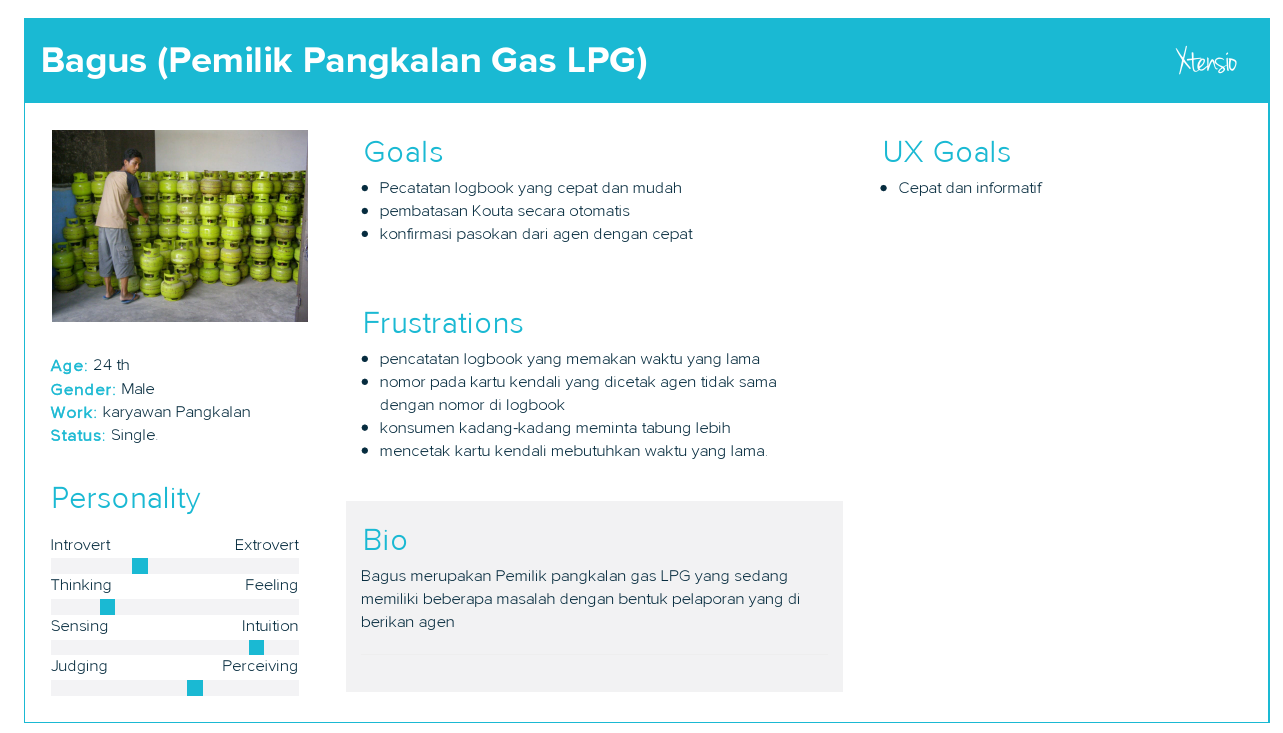
\includegraphics [width = 15cm]{gambar/persona/pangkalan}
\end{figure}
%-----------------------------------------------------------------------------%
\addcontentsline{toc}{chapter}{LAMPIRAN 2}
\chapter*{Lampiran 2}
\newappendix{Lampiran 2. Kuesioner SUS}
\begin{figure}[H]
	\center
	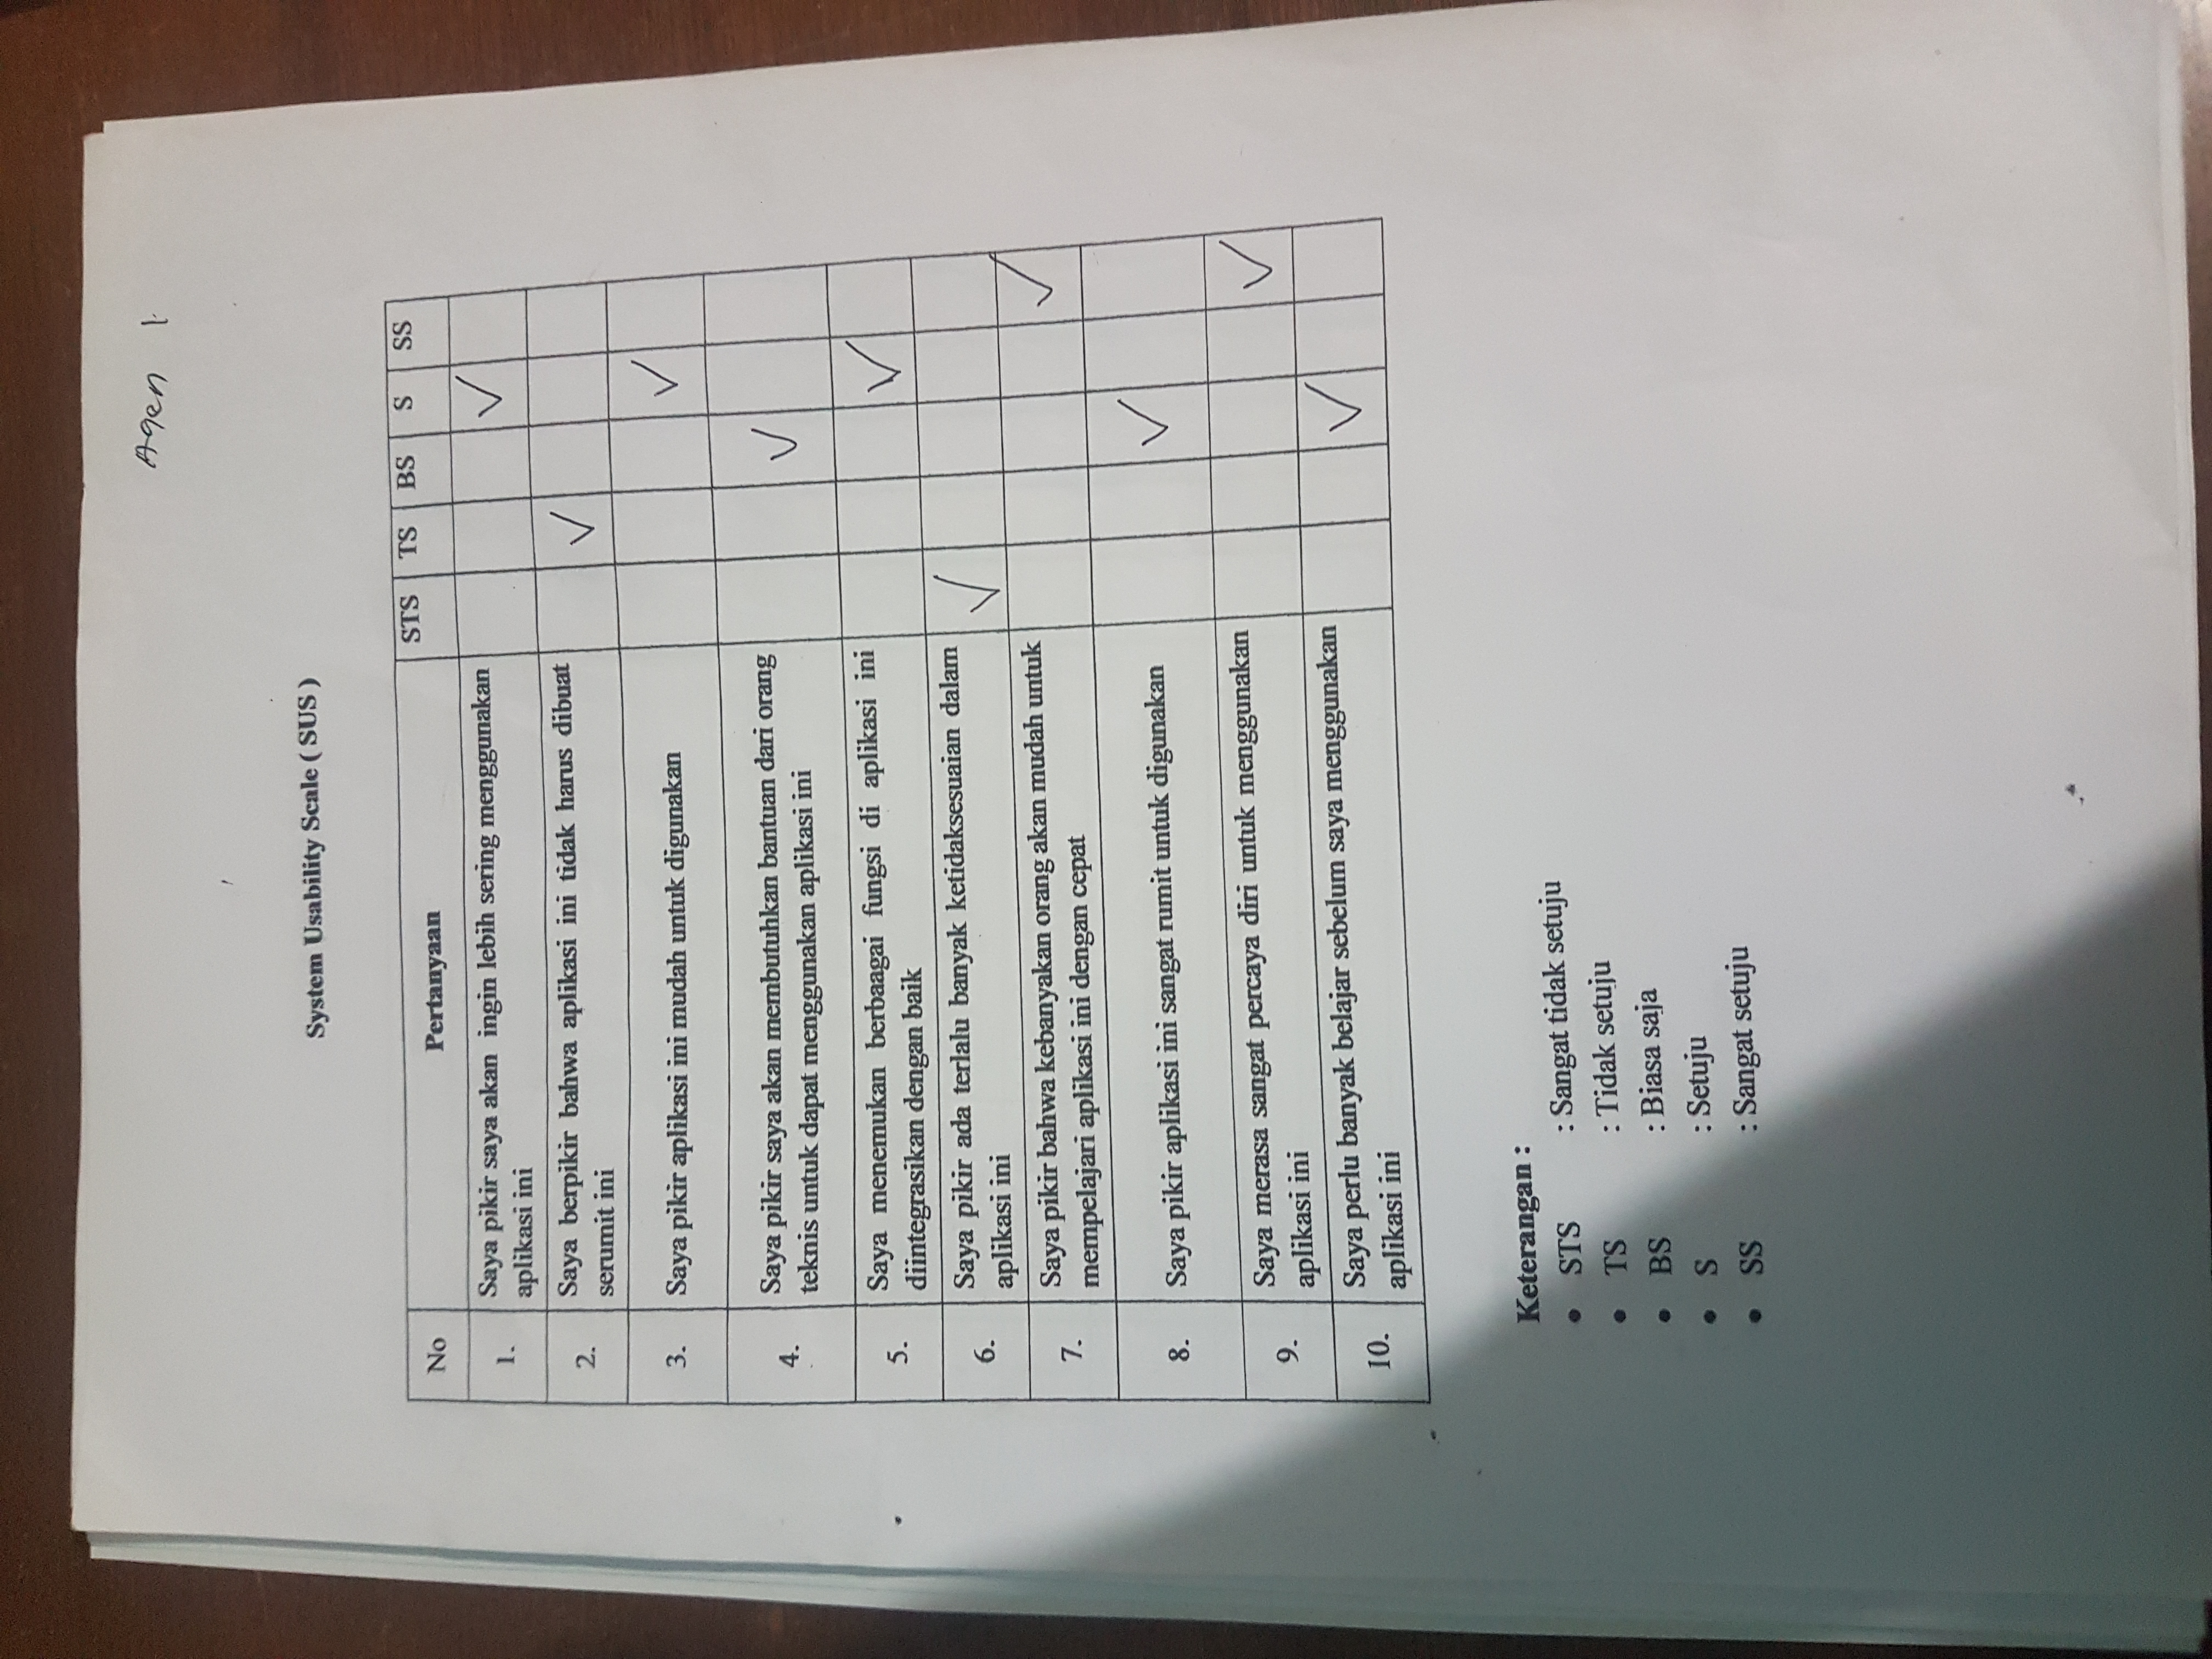
\includegraphics [width = 17cm,angle=-90]{gambar/pengujian/agen1}
\end{figure}
\begin{figure}[H]
	\center
	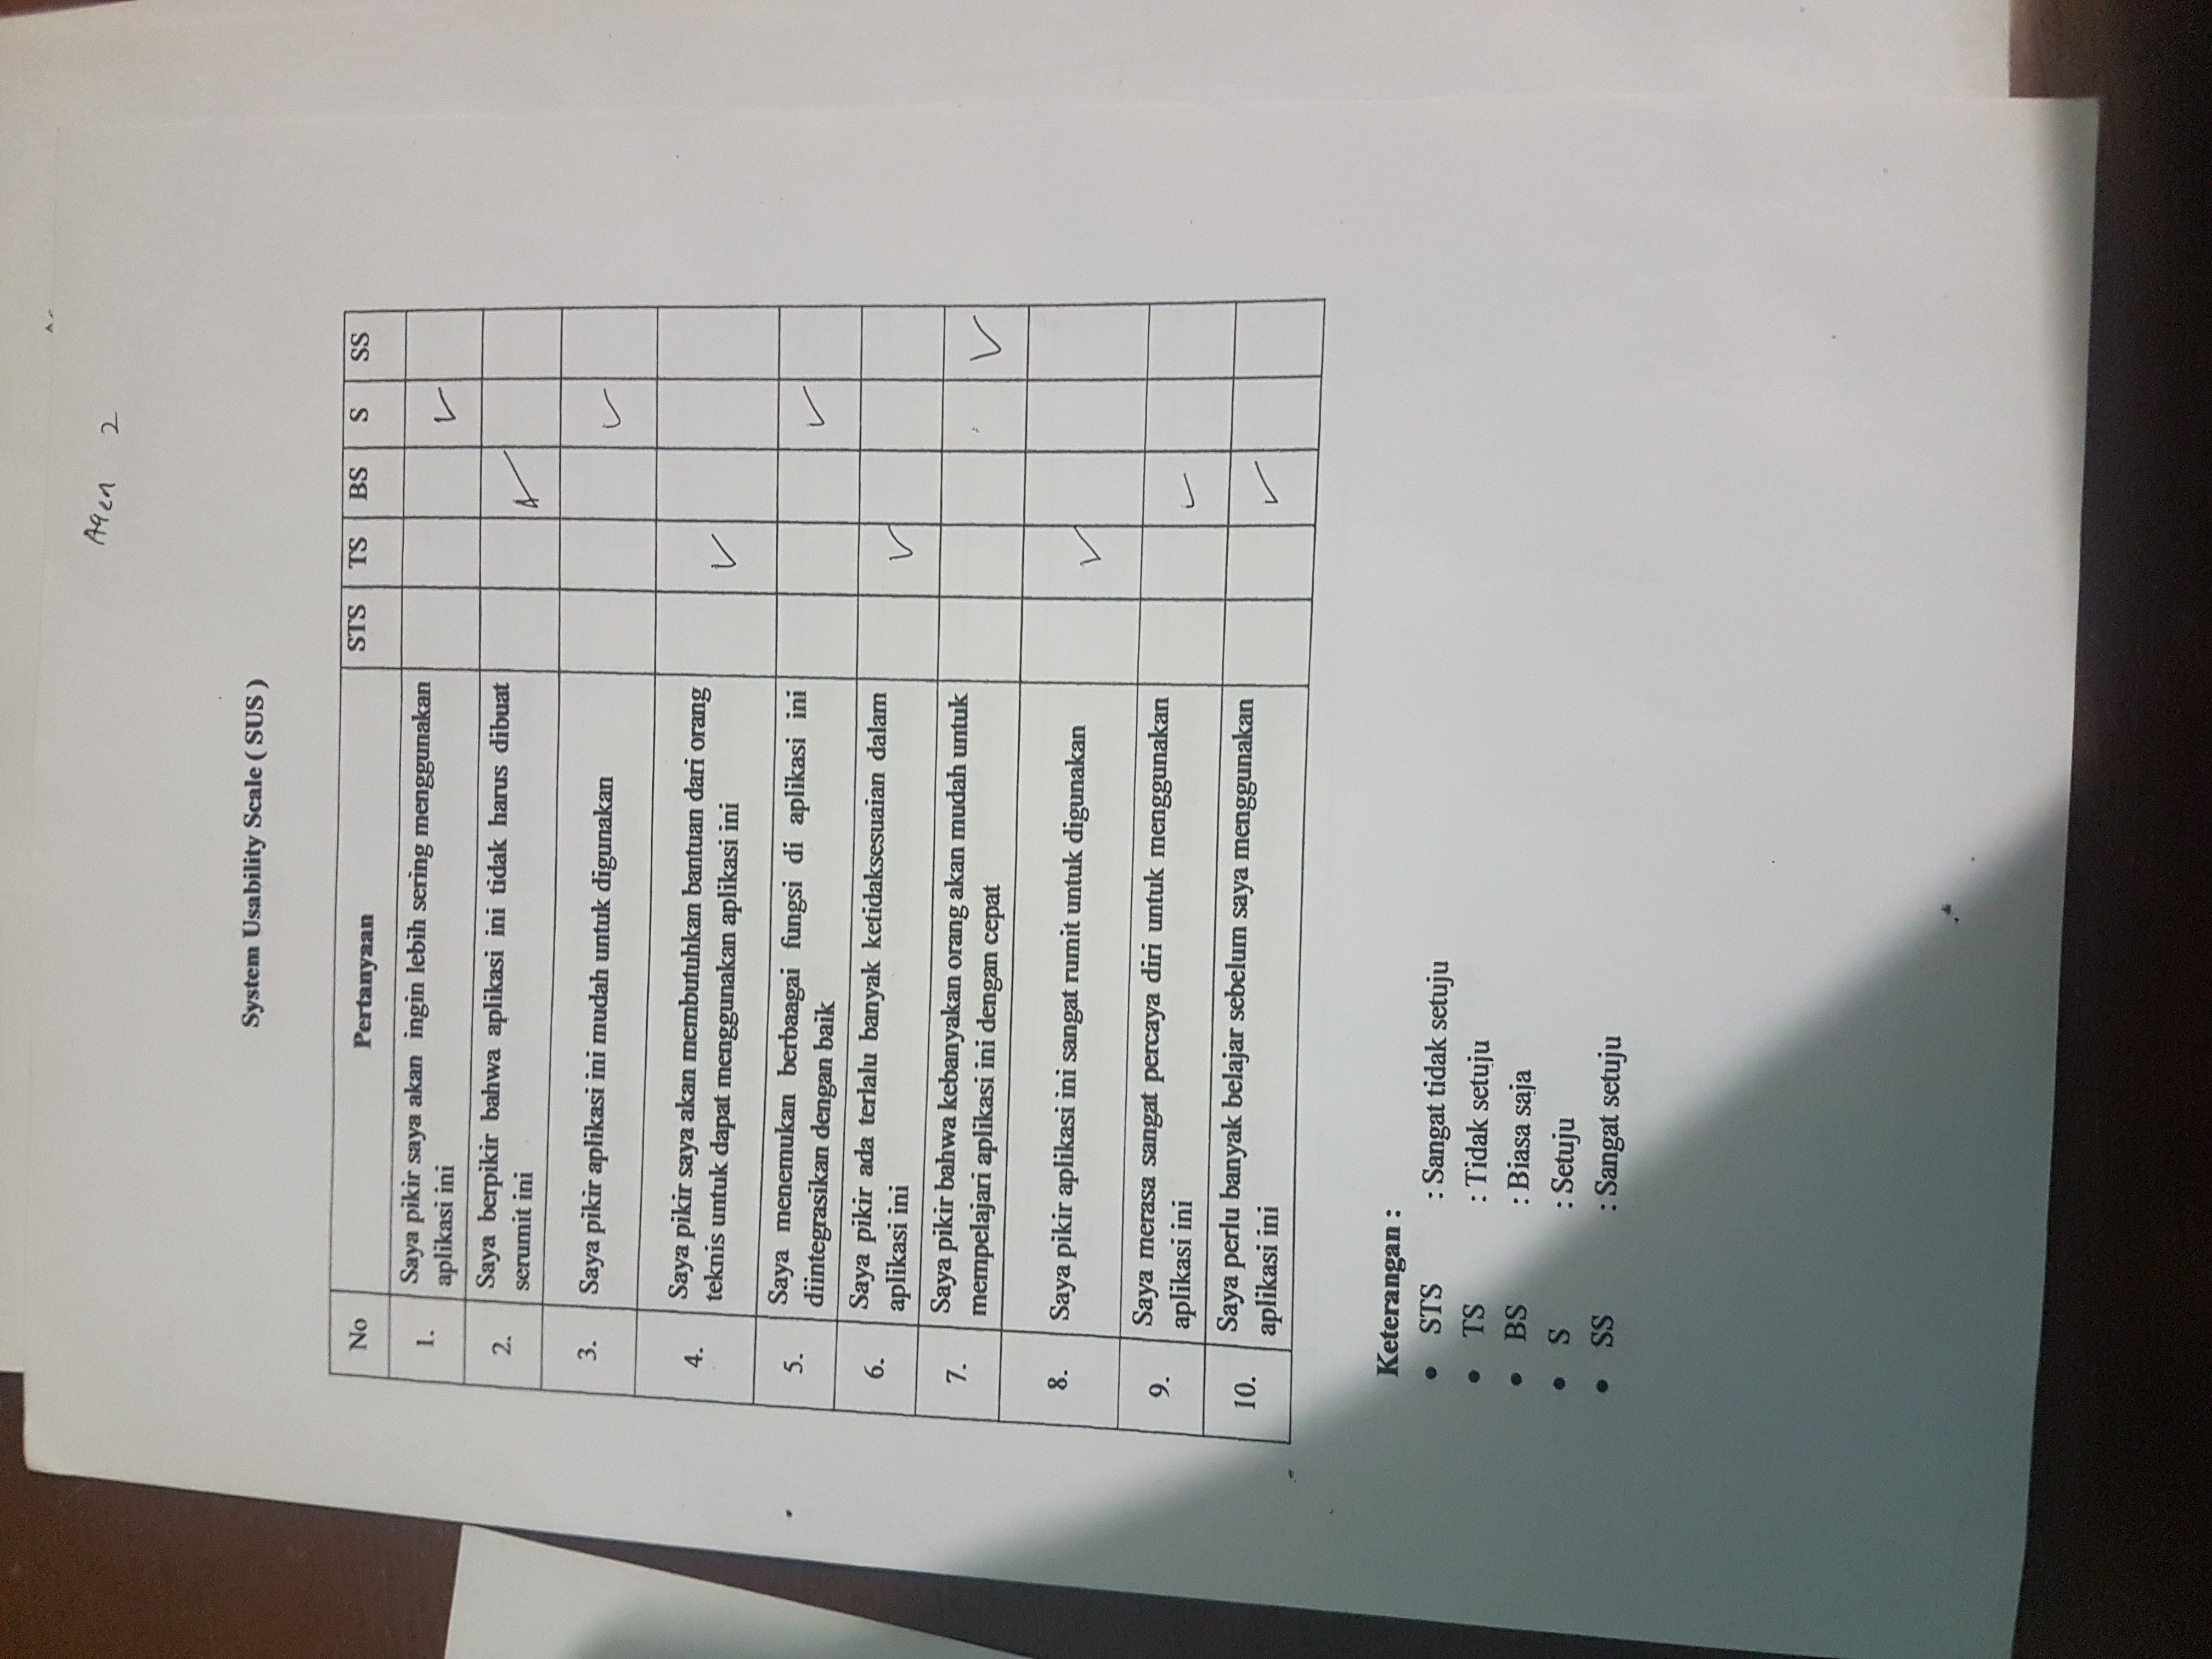
\includegraphics [width = 17cm,angle=-90]{gambar/pengujian/agen2}
\end{figure}
\begin{figure}[H]
	\center
	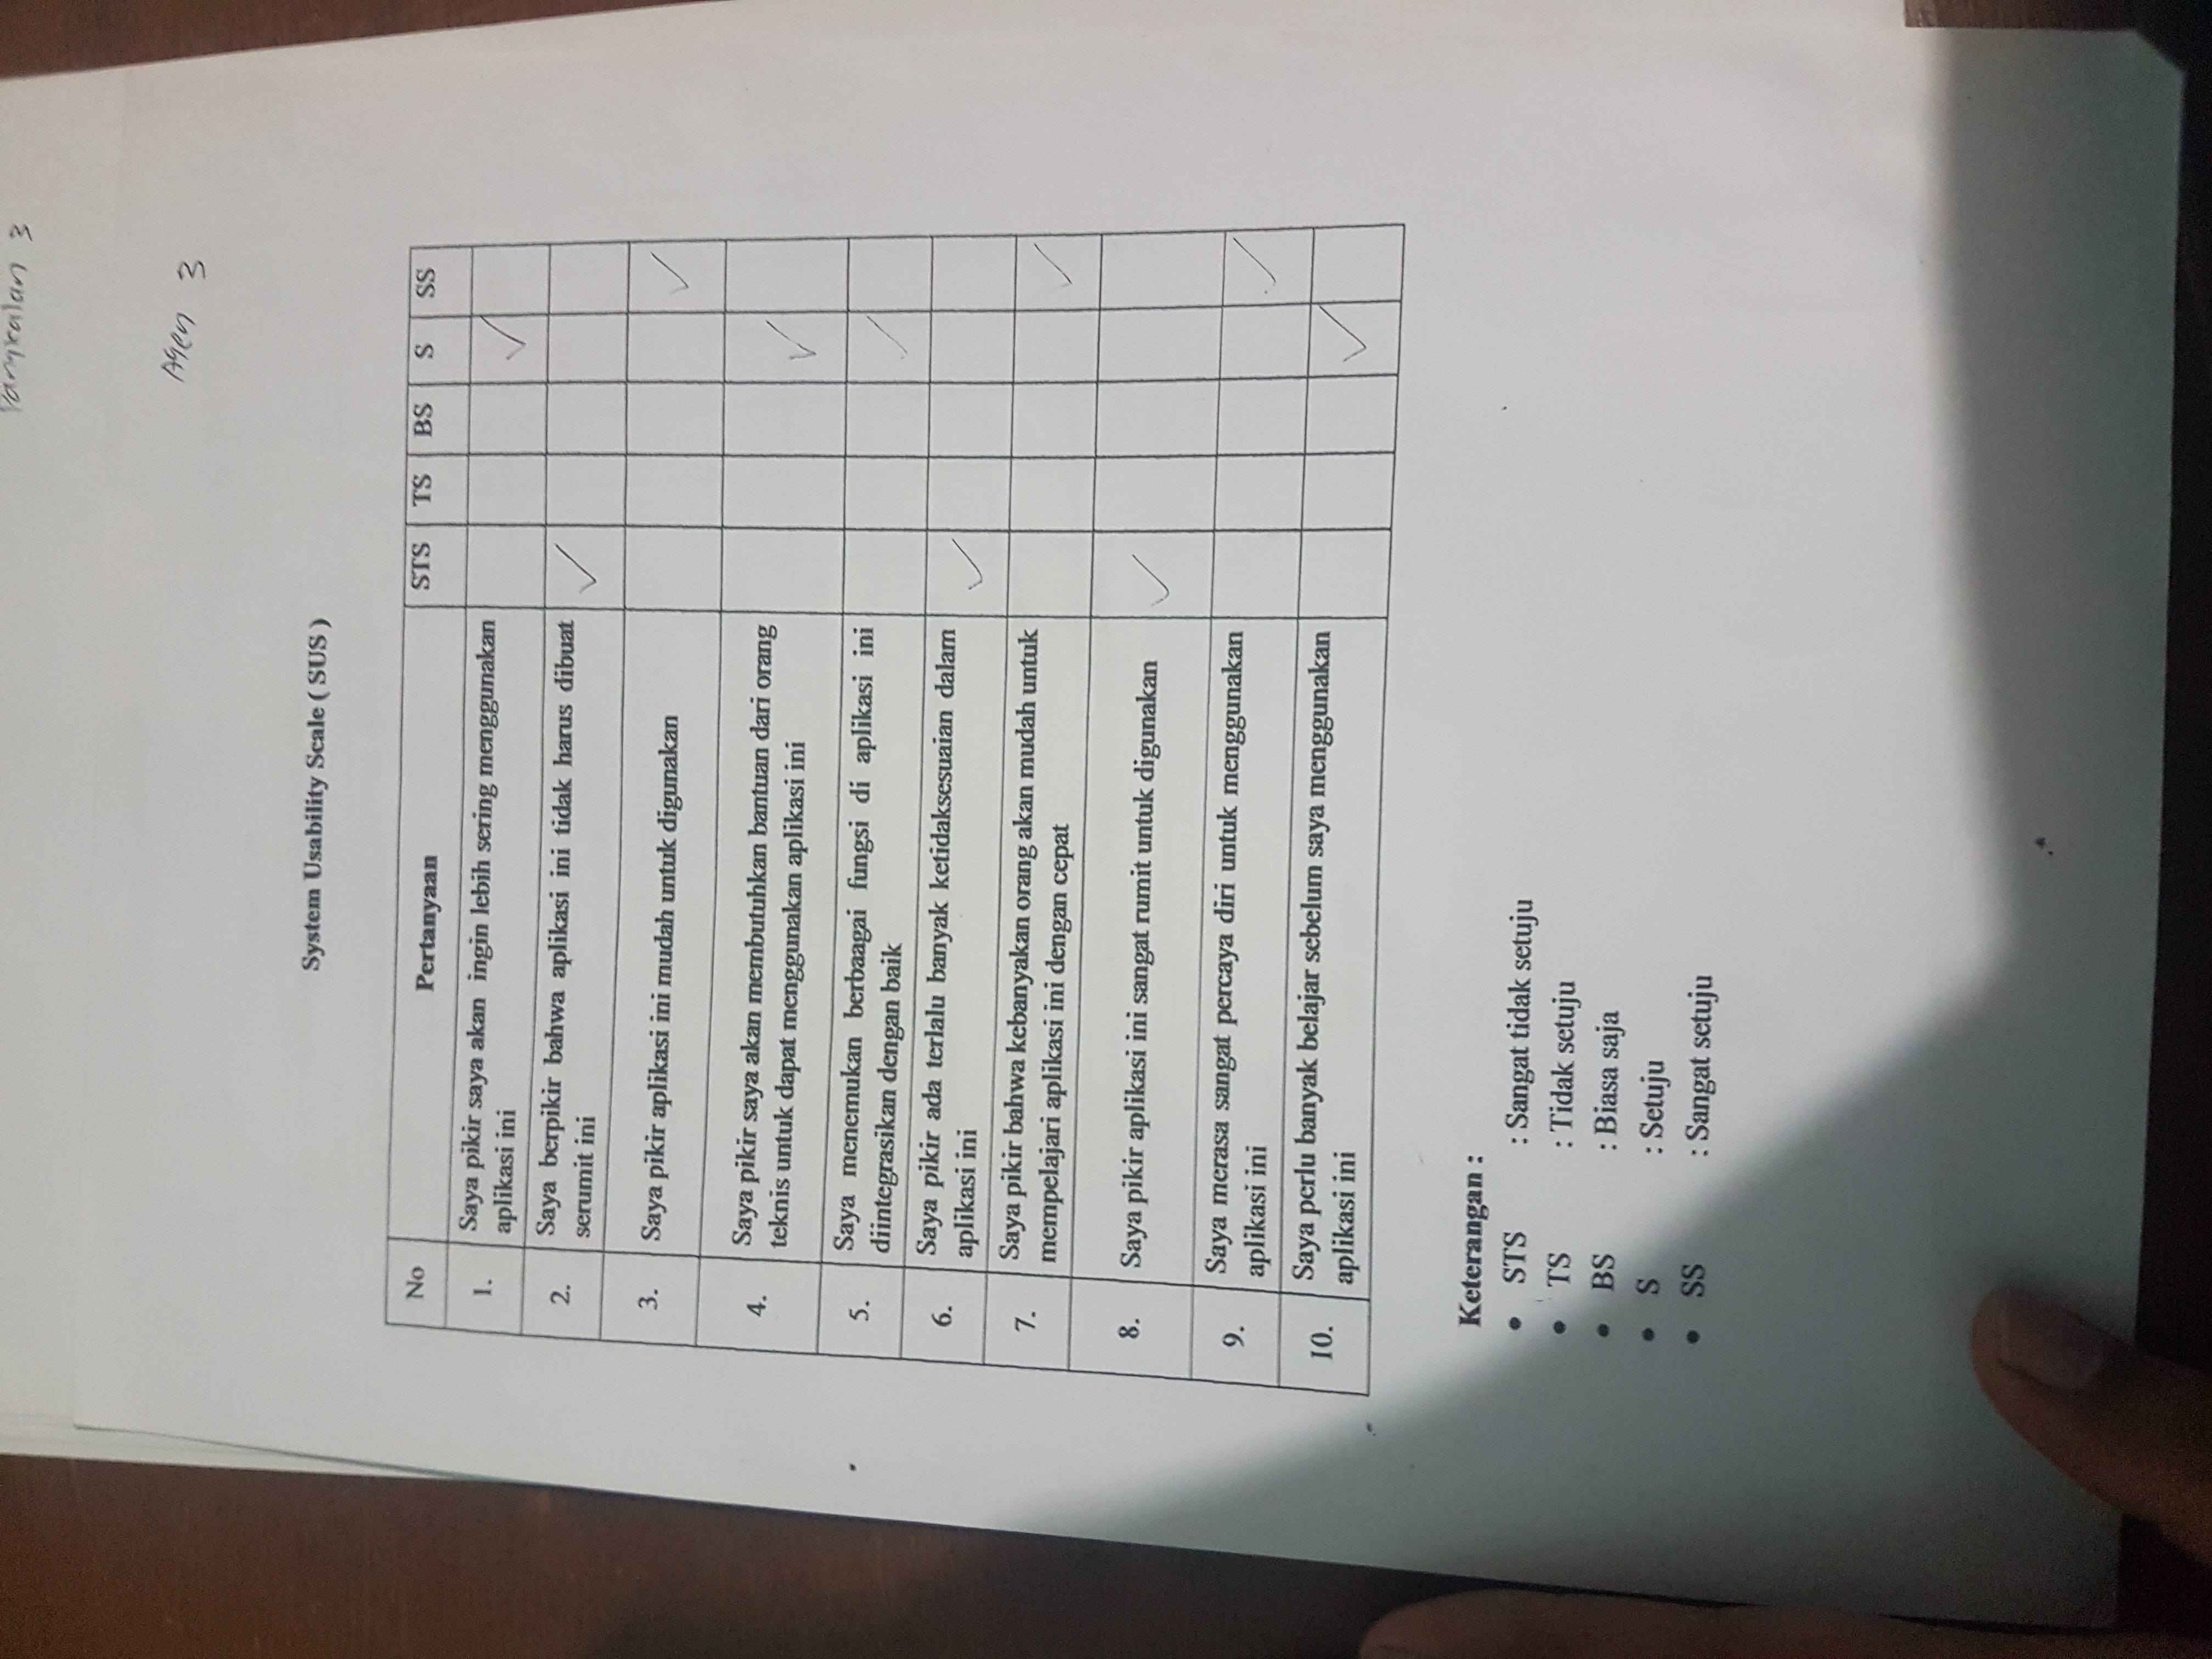
\includegraphics [width = 17cm,angle=-90]{gambar/pengujian/agen3}
\end{figure}
\begin{figure}[H]
	\center
	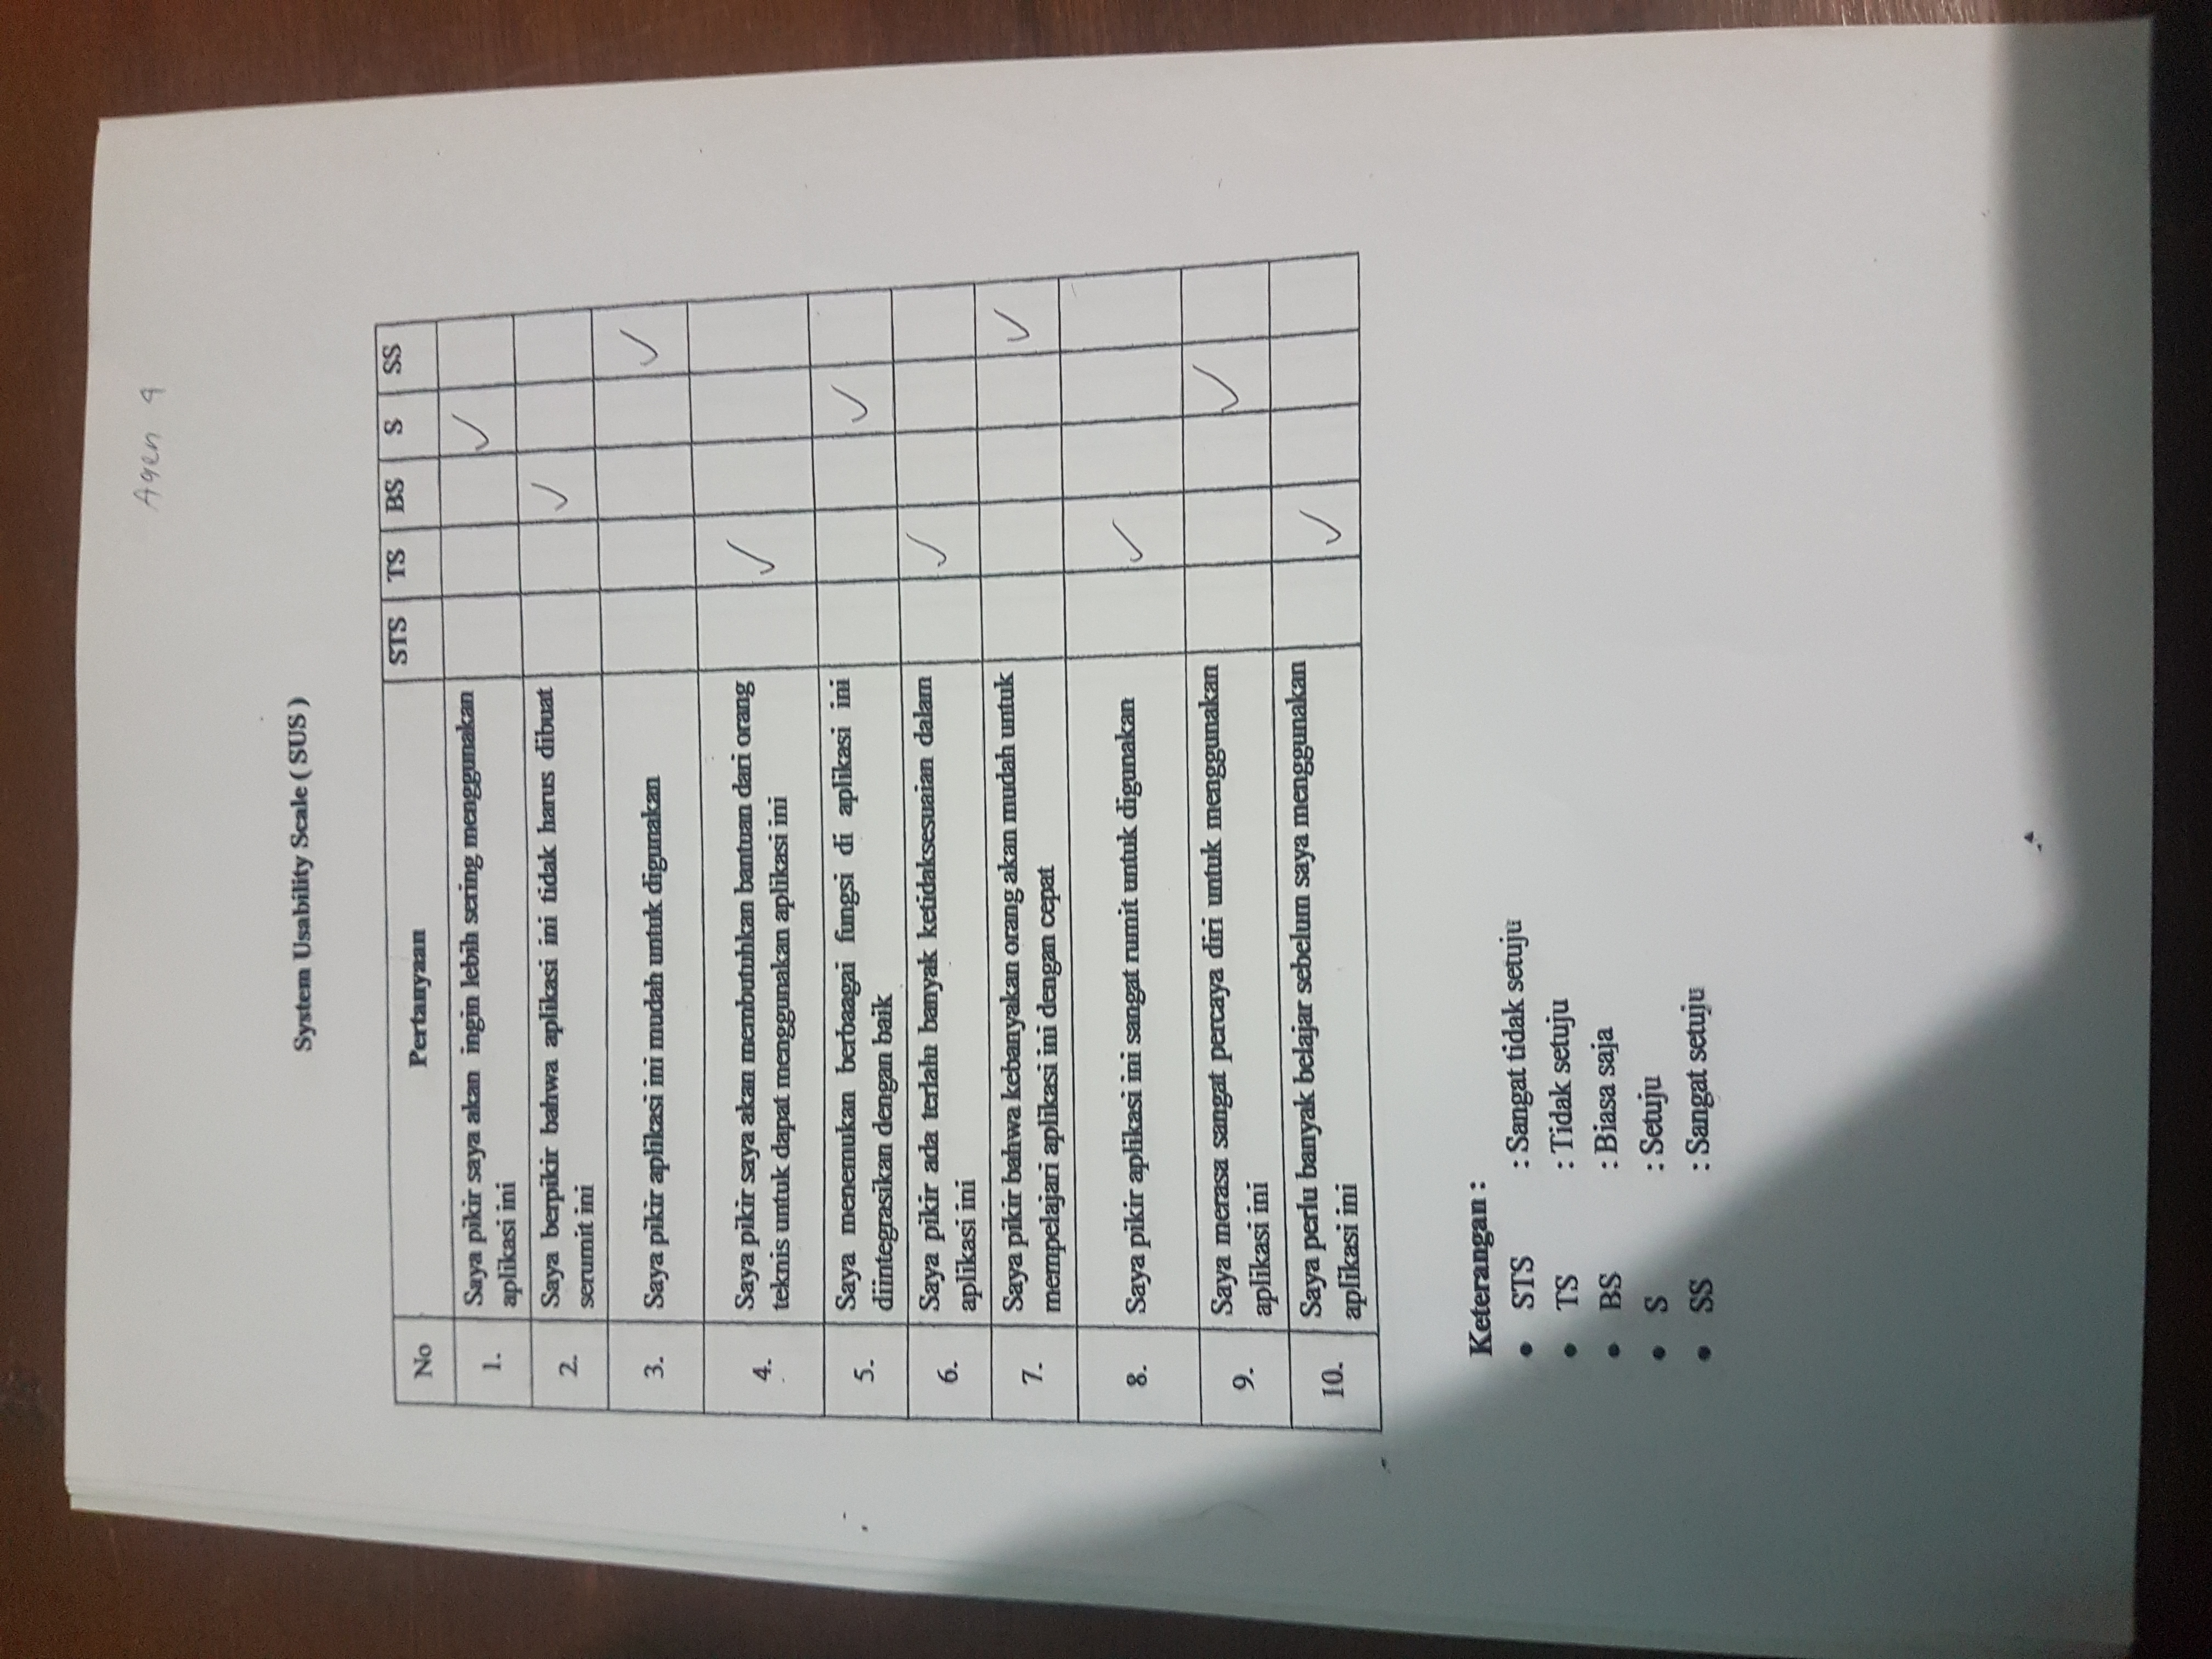
\includegraphics [width = 17cm,angle=-90]{gambar/pengujian/agen4}
\end{figure}
\begin{figure}[H]
	\center
	\includegraphics [width = 17cm,angle=-90]{gambar/pengujian/agen5}
\end{figure}
\begin{figure}[H]
	\center
	\includegraphics [width = 17cm,angle=-90]{gambar/pengujian/agen6}
\end{figure}
\begin{figure}[H]
	\center
	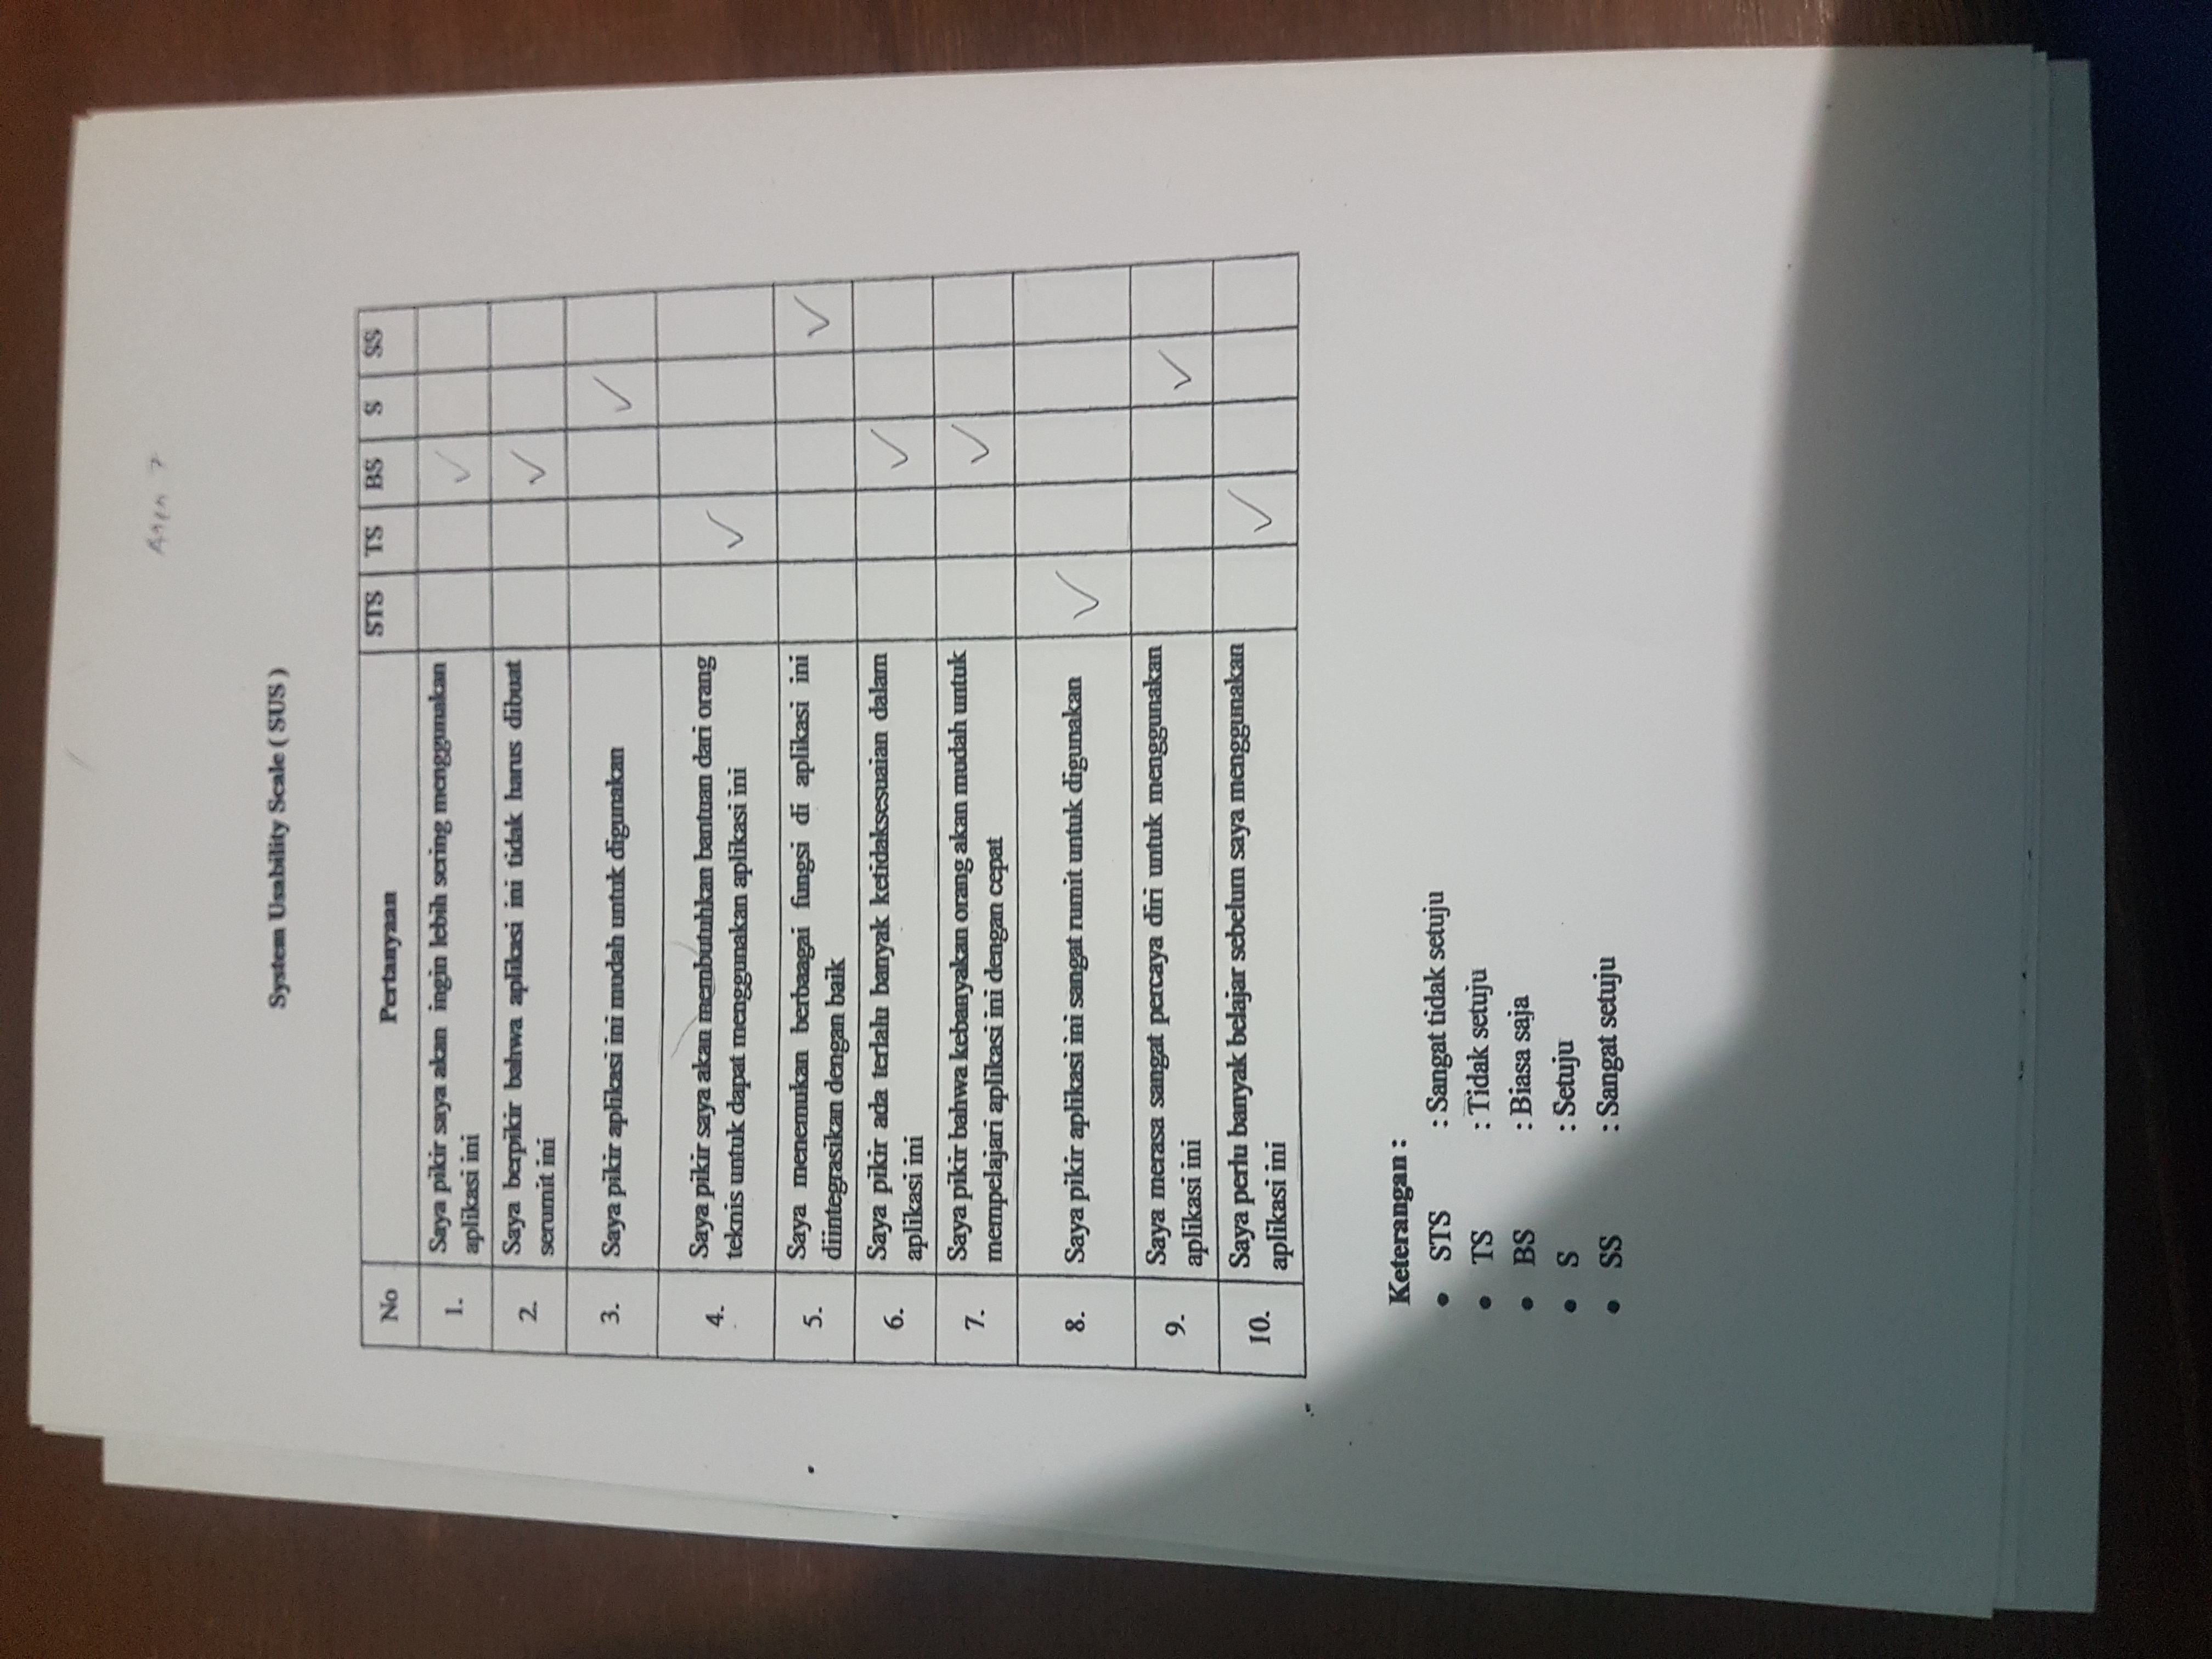
\includegraphics [width = 17cm,angle=-90]{gambar/pengujian/agen7}
\end{figure}
\begin{figure}[H]
	\center
	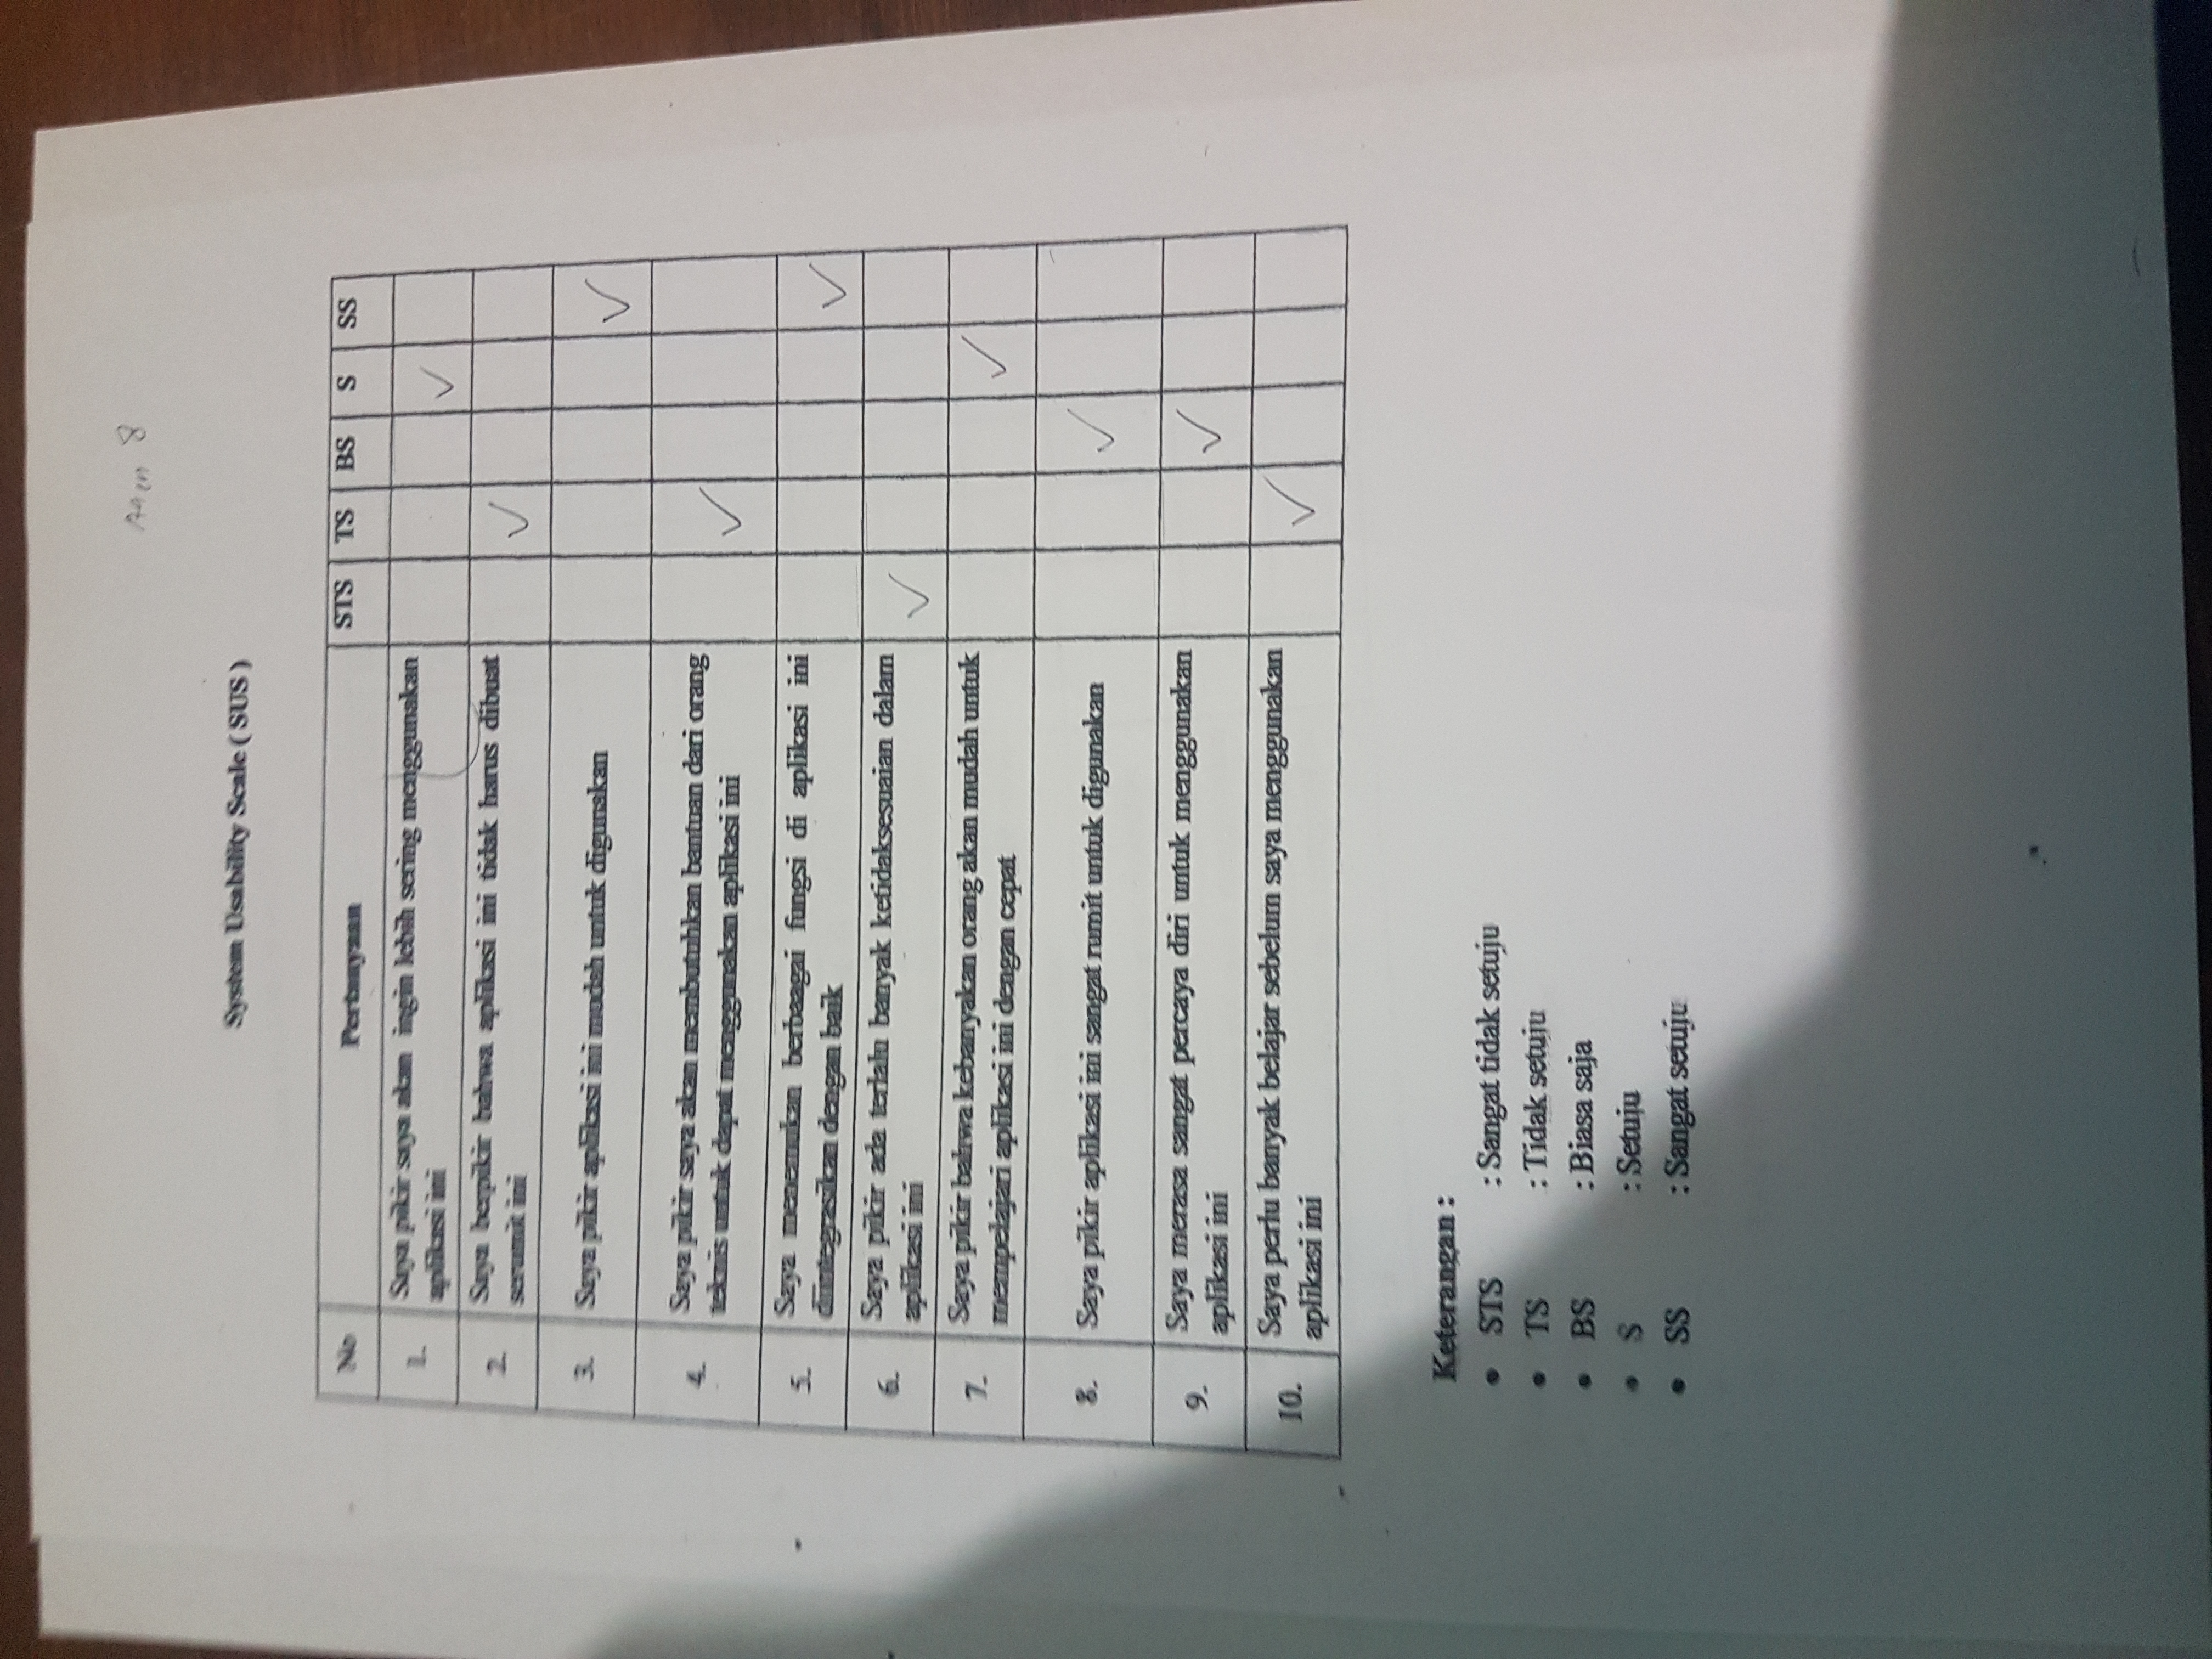
\includegraphics [width = 17cm,angle=-90]{gambar/pengujian/agen8}
\end{figure}

\begin{figure}[H]
	\center
	\includegraphics [width = 17cm,angle=-90]{gambar/pengujian/pangkalan1}
\end{figure}

\begin{figure}[H]
	\center
	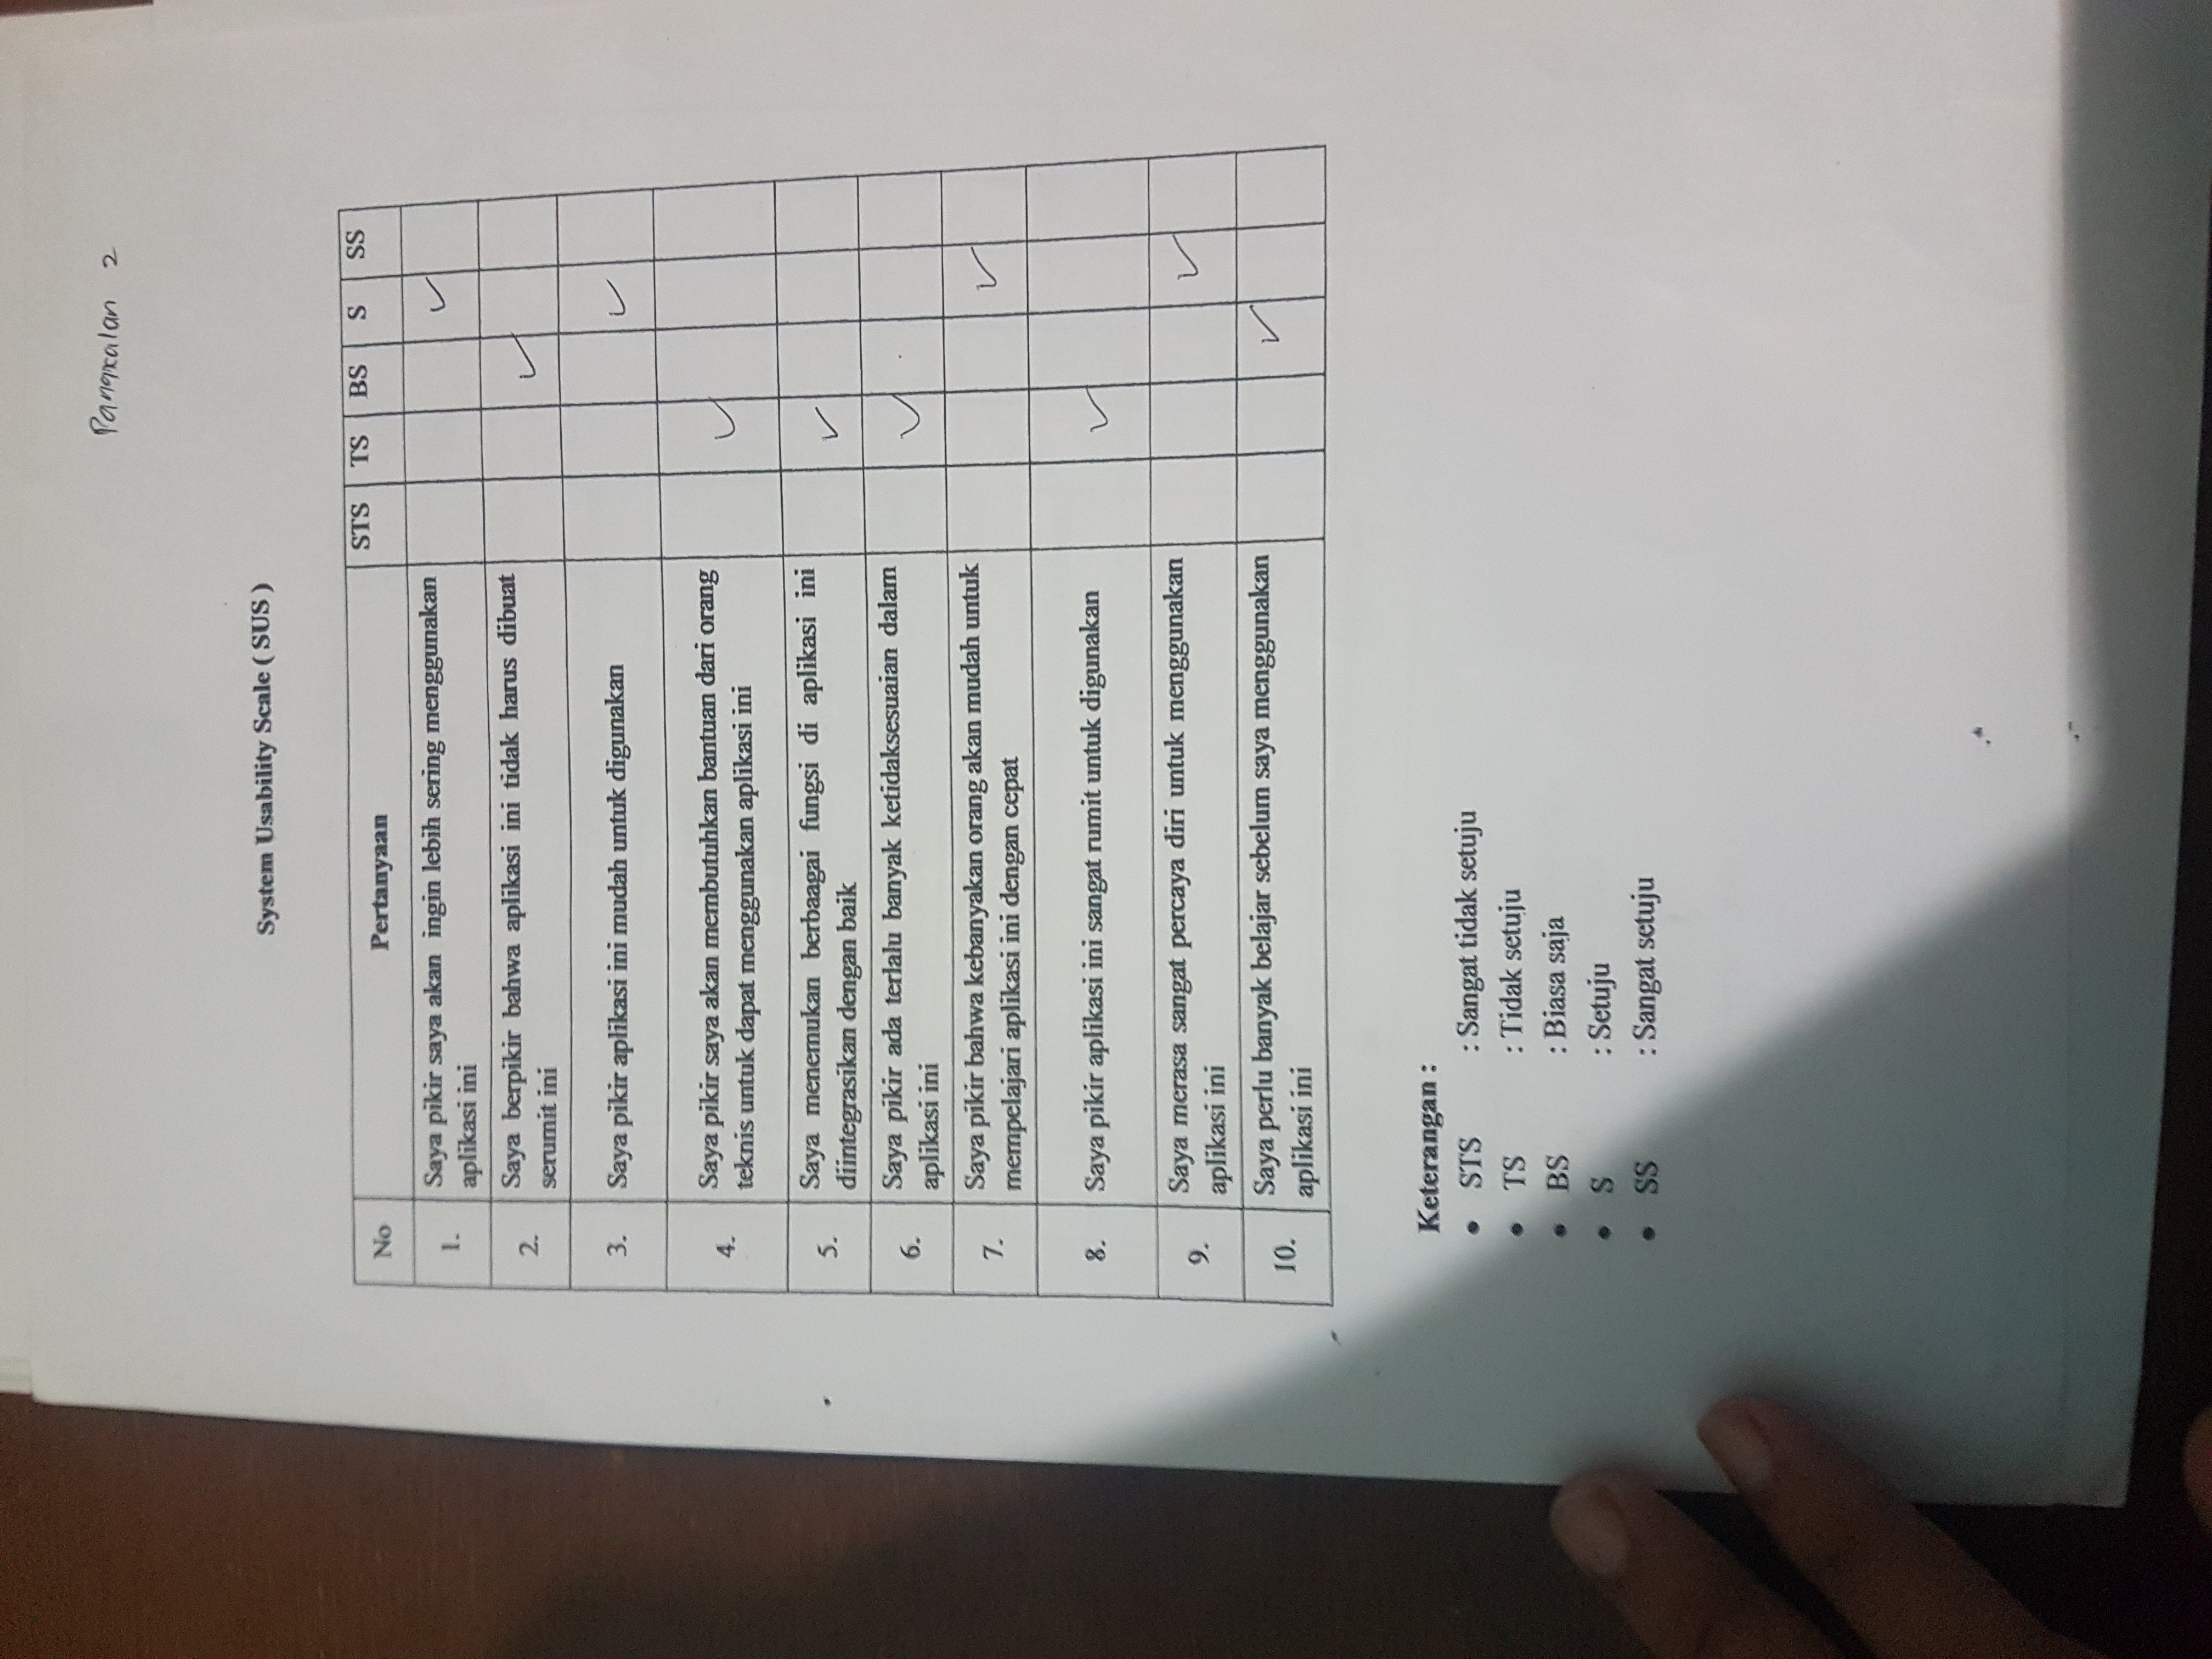
\includegraphics [width = 17cm,angle=-90]{gambar/pengujian/pangkalan2}
\end{figure}
\begin{figure}[H]
	\center
	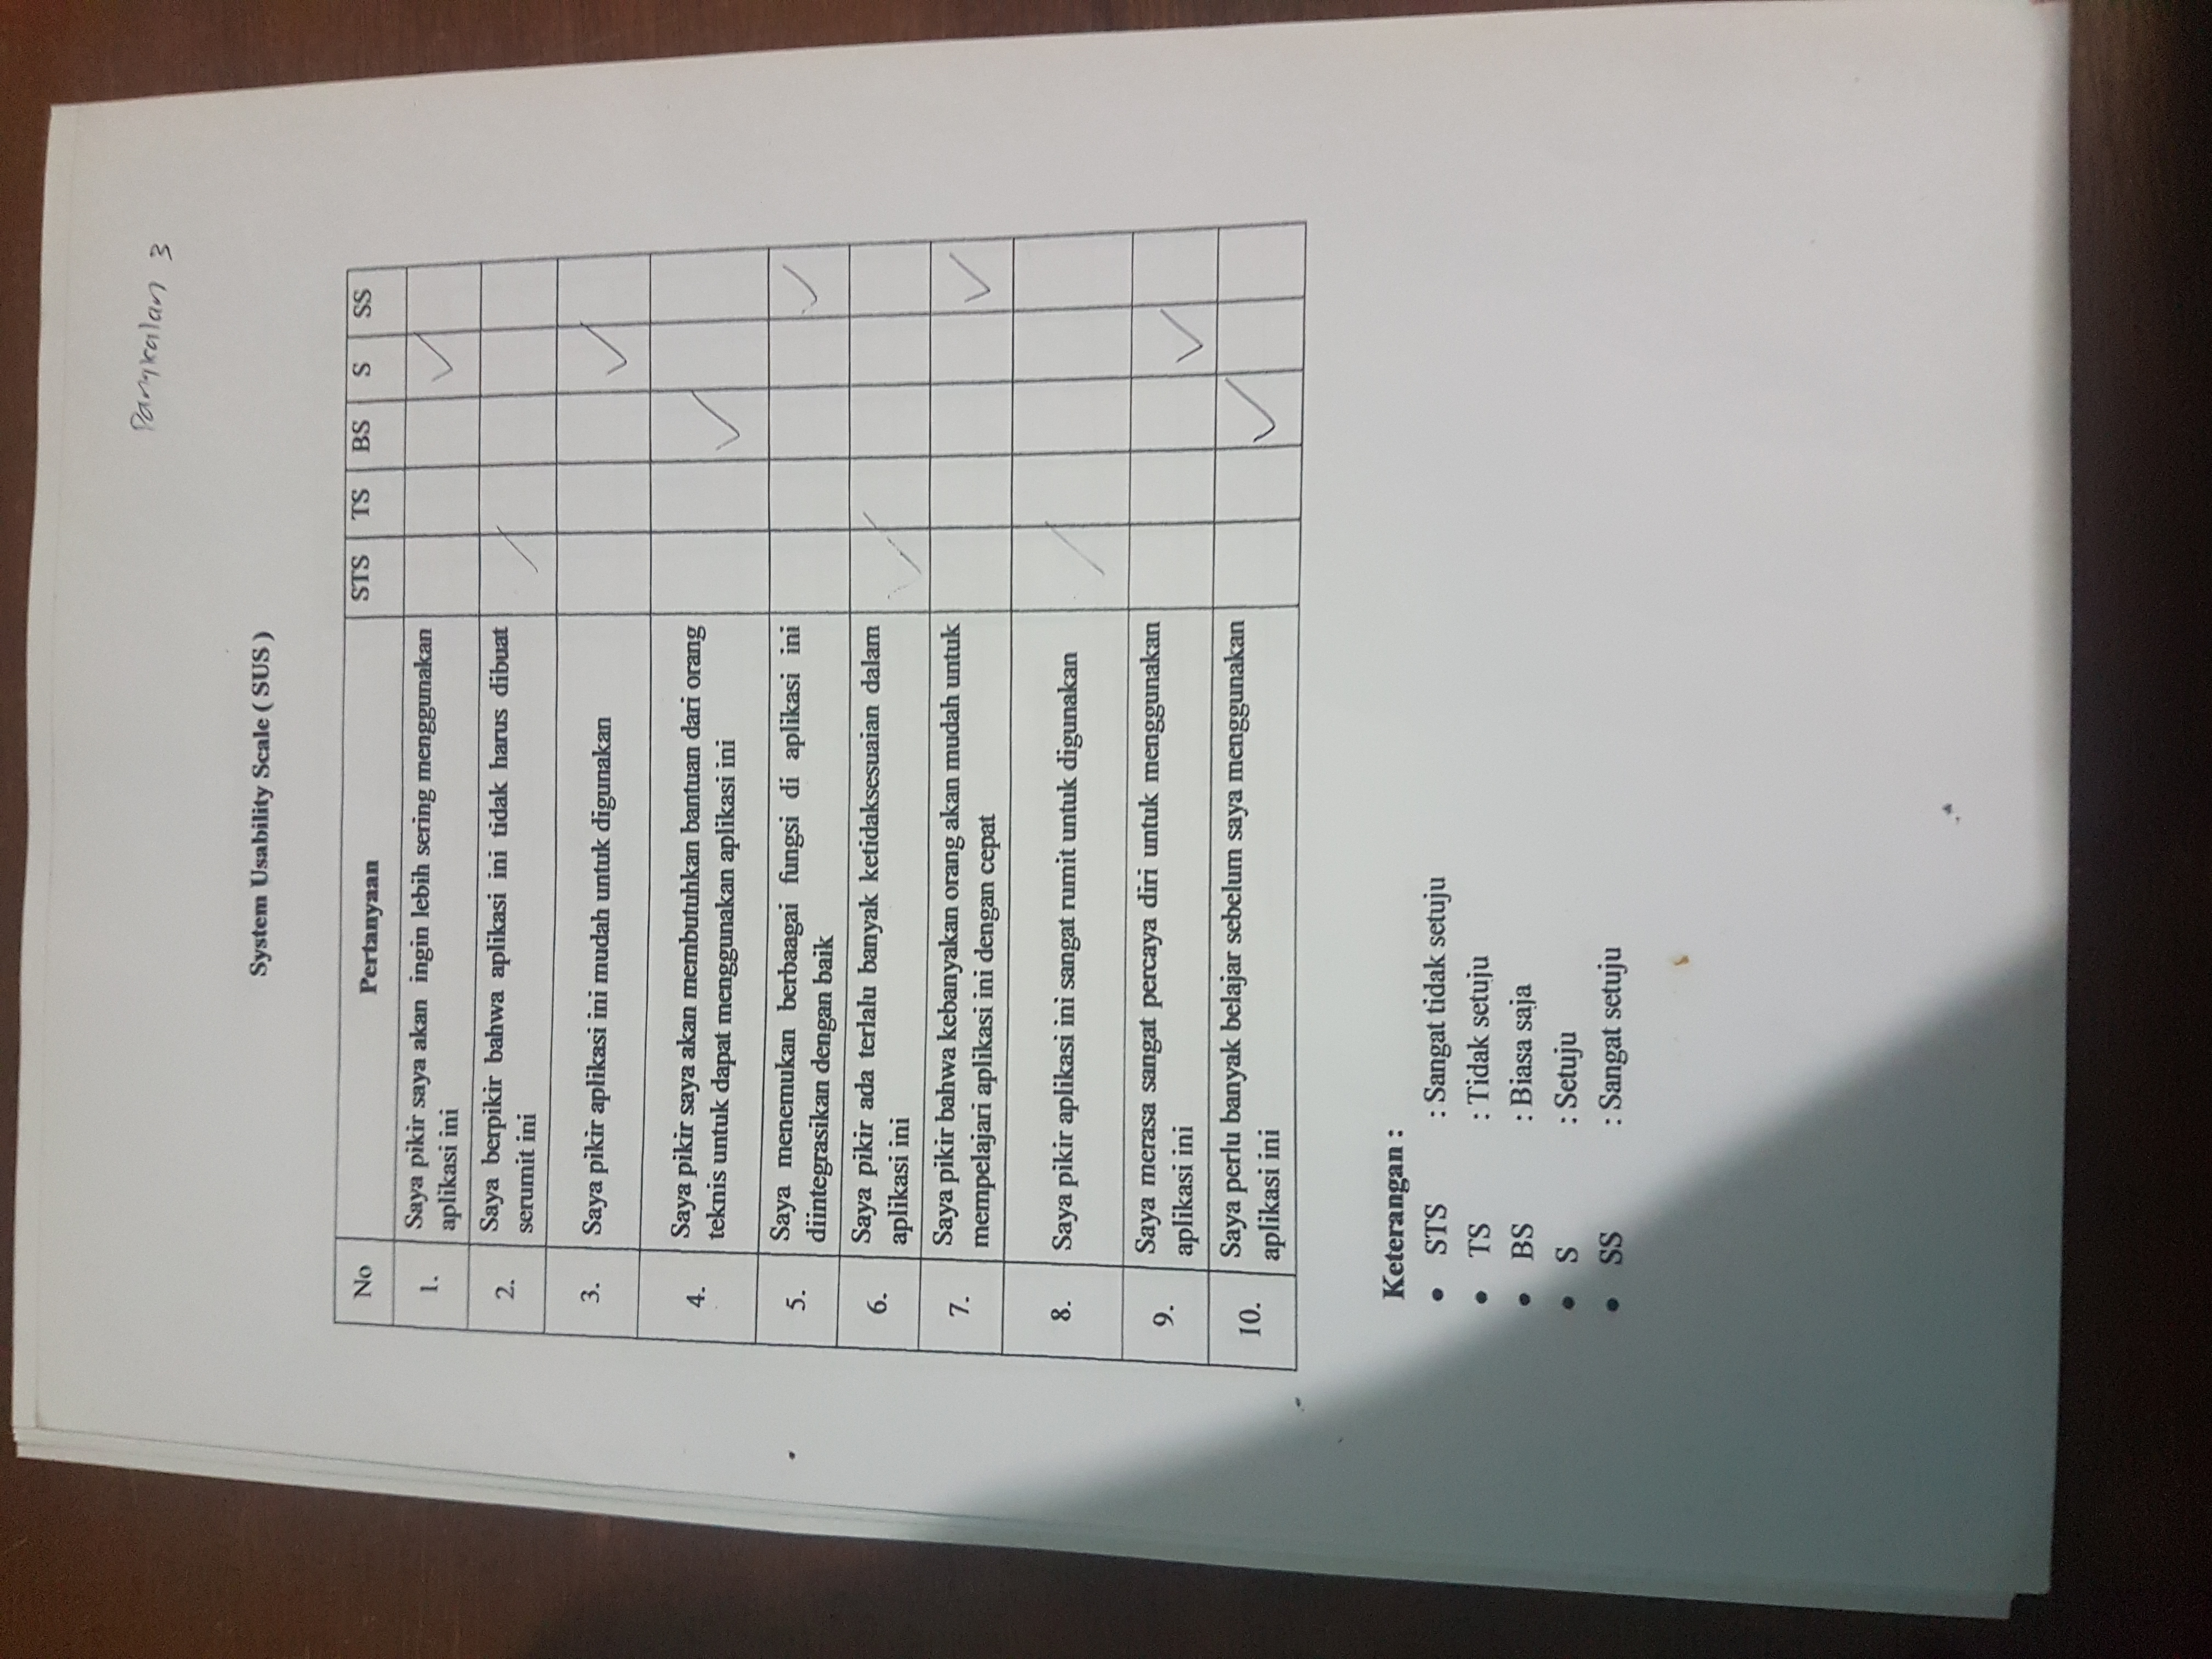
\includegraphics [width = 17cm,angle=-90]{gambar/pengujian/pangkalan3}
\end{figure}
\begin{figure}[H]
	\center
	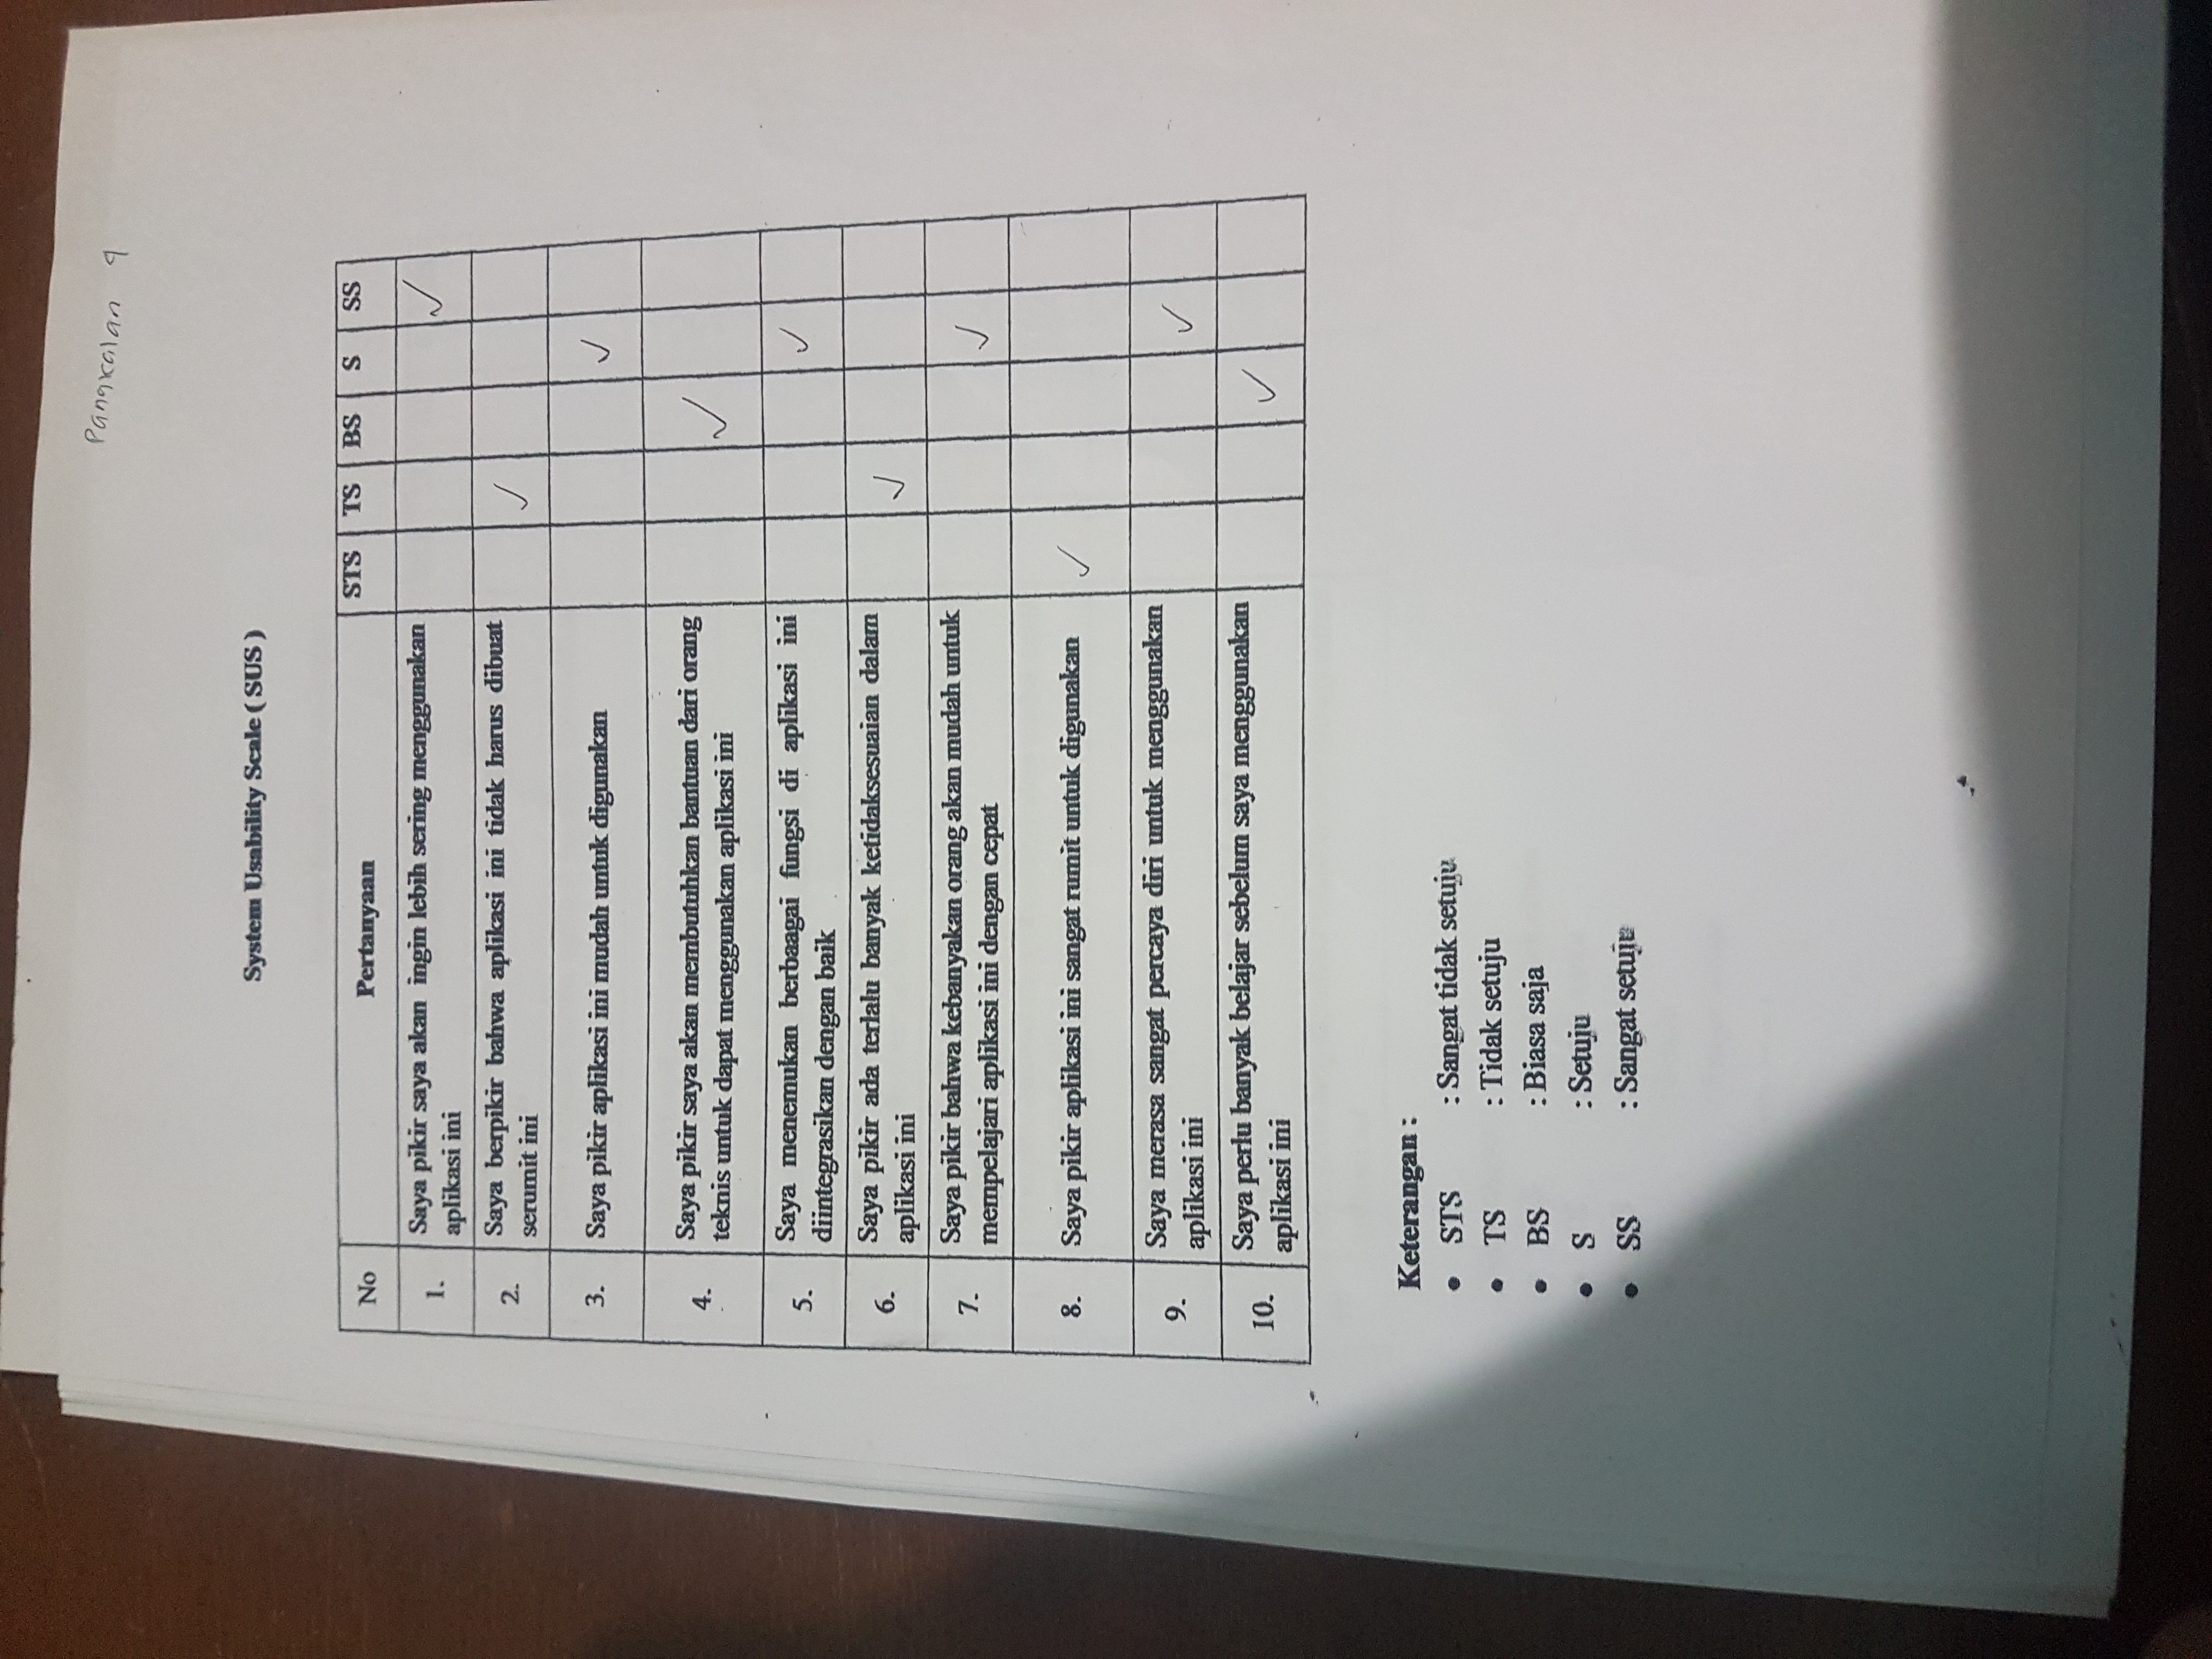
\includegraphics [width = 17cm,angle=-90]{gambar/pengujian/pangkalan4}
\end{figure}
\begin{figure}[H]
	\center
	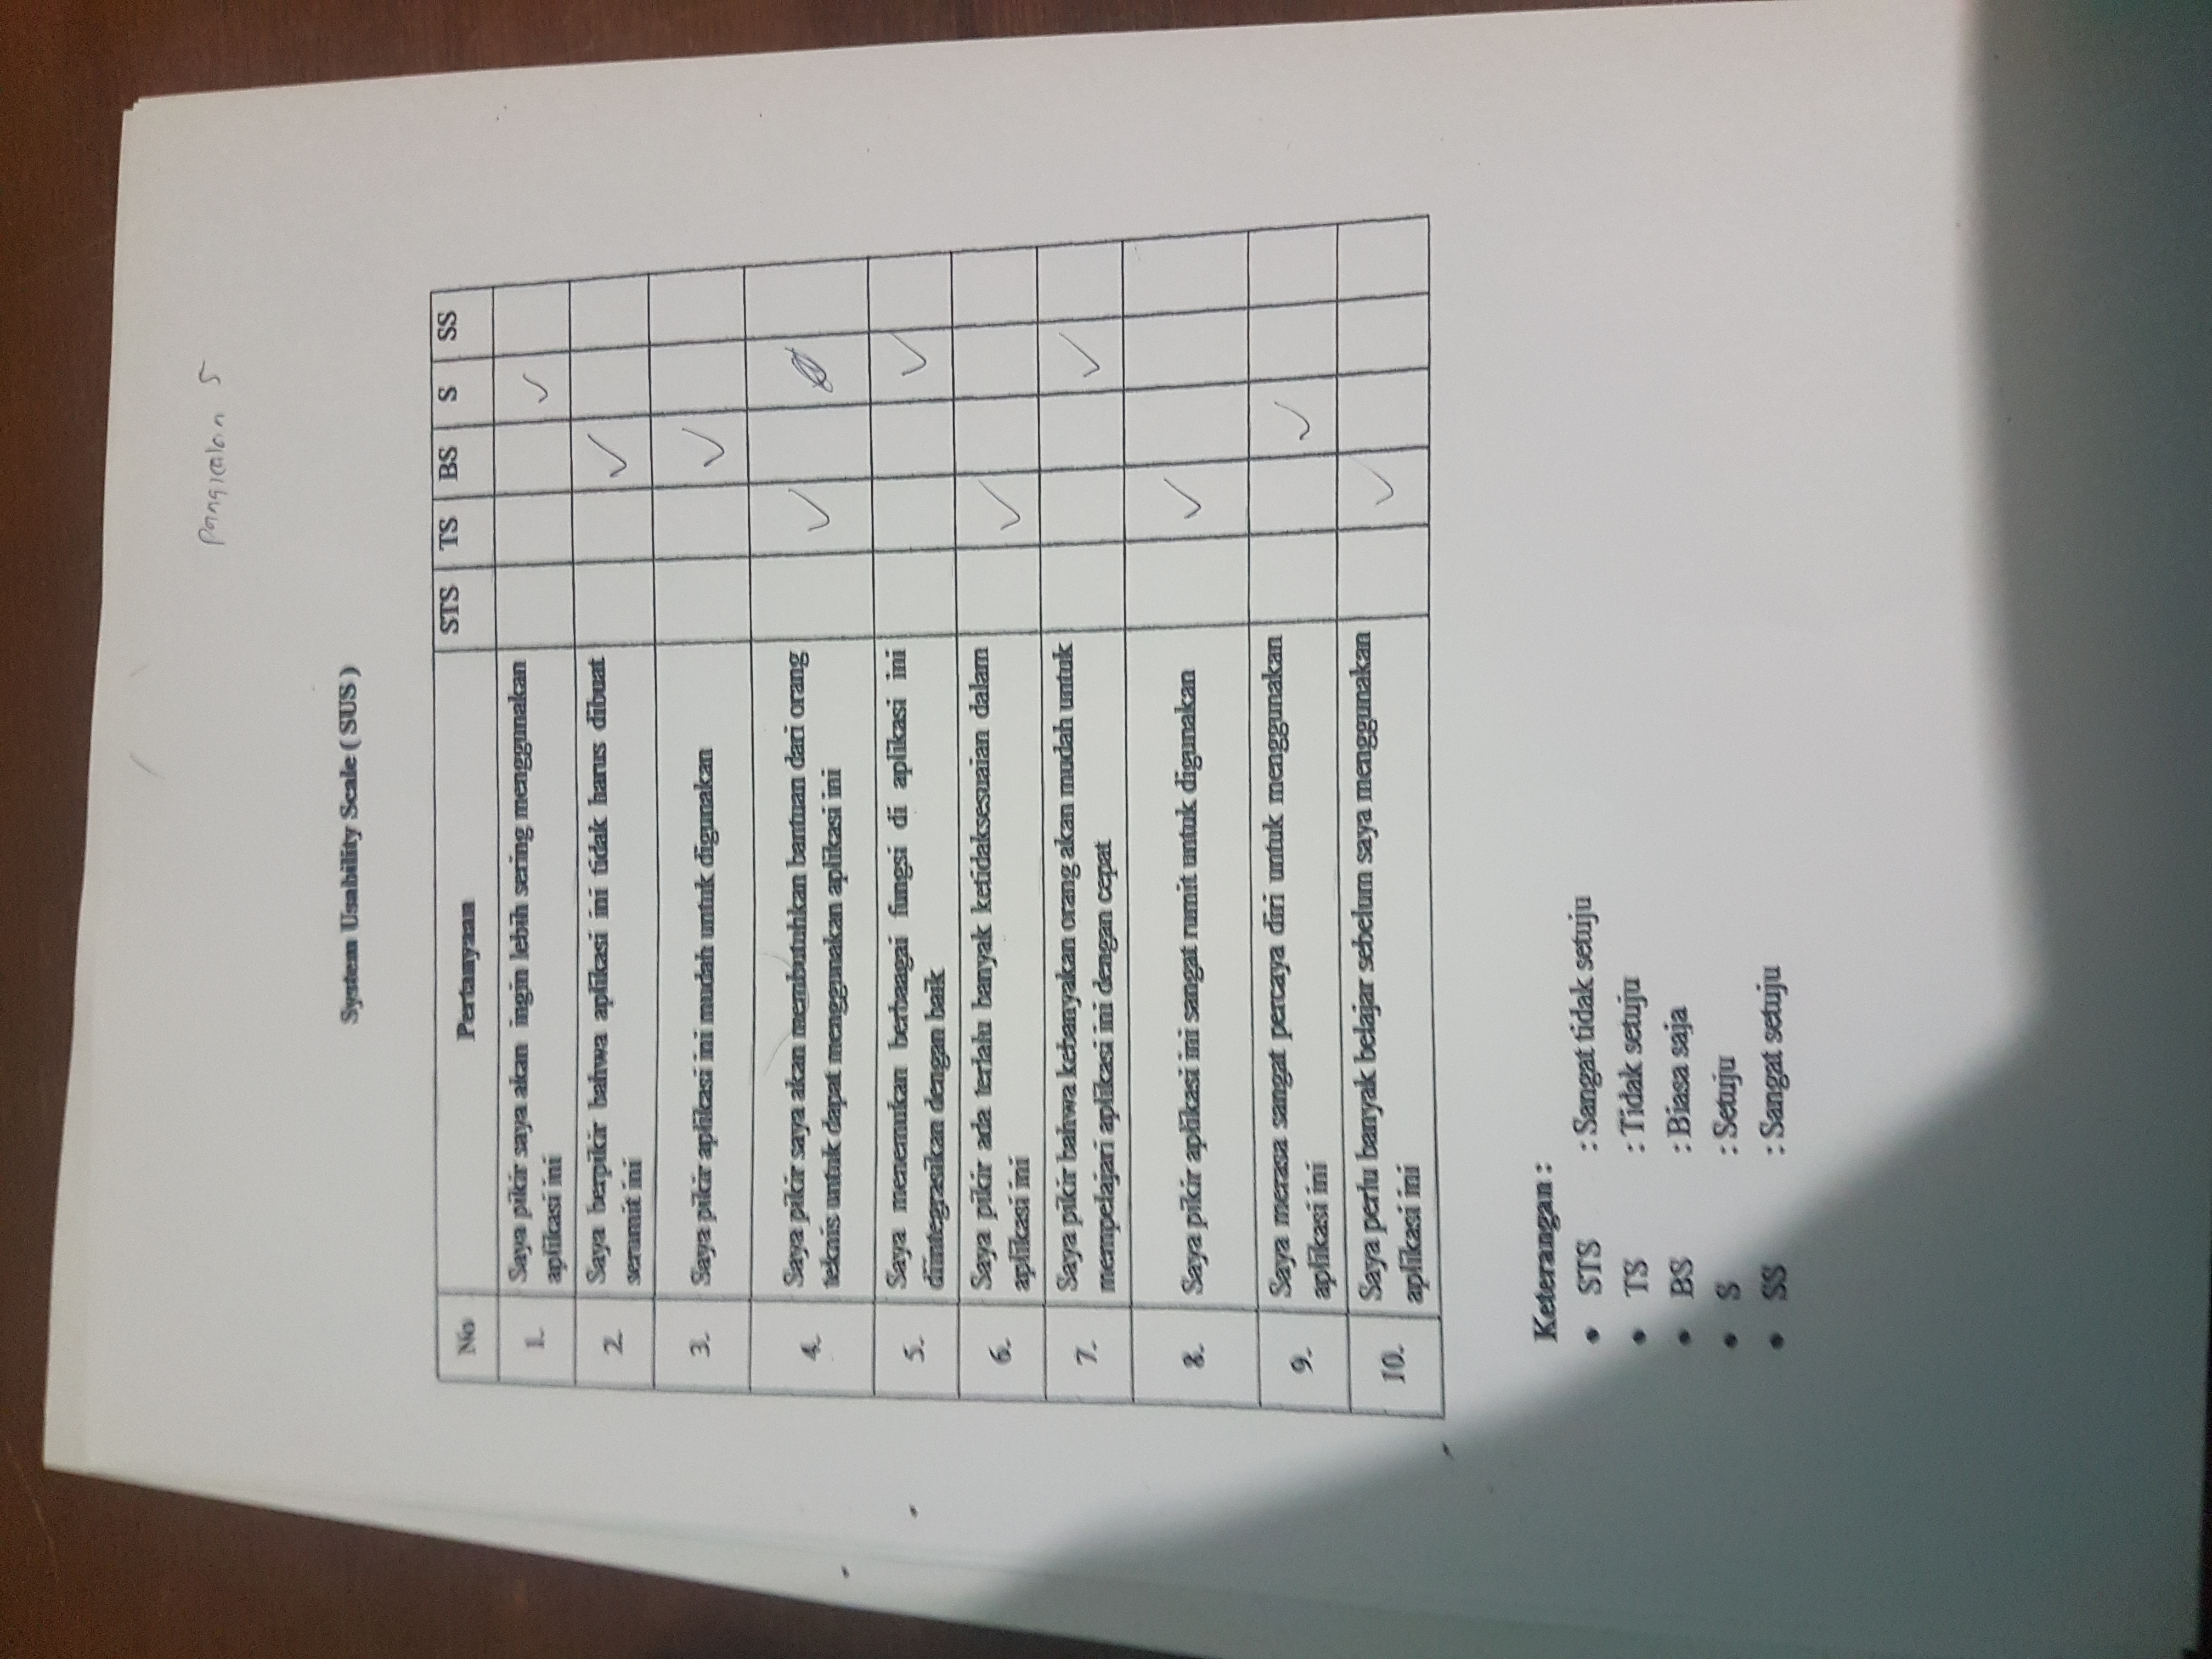
\includegraphics [width = 17cm,angle=-90]{gambar/pengujian/pangkalan5}
\end{figure}
\begin{figure}[H]
	\center
	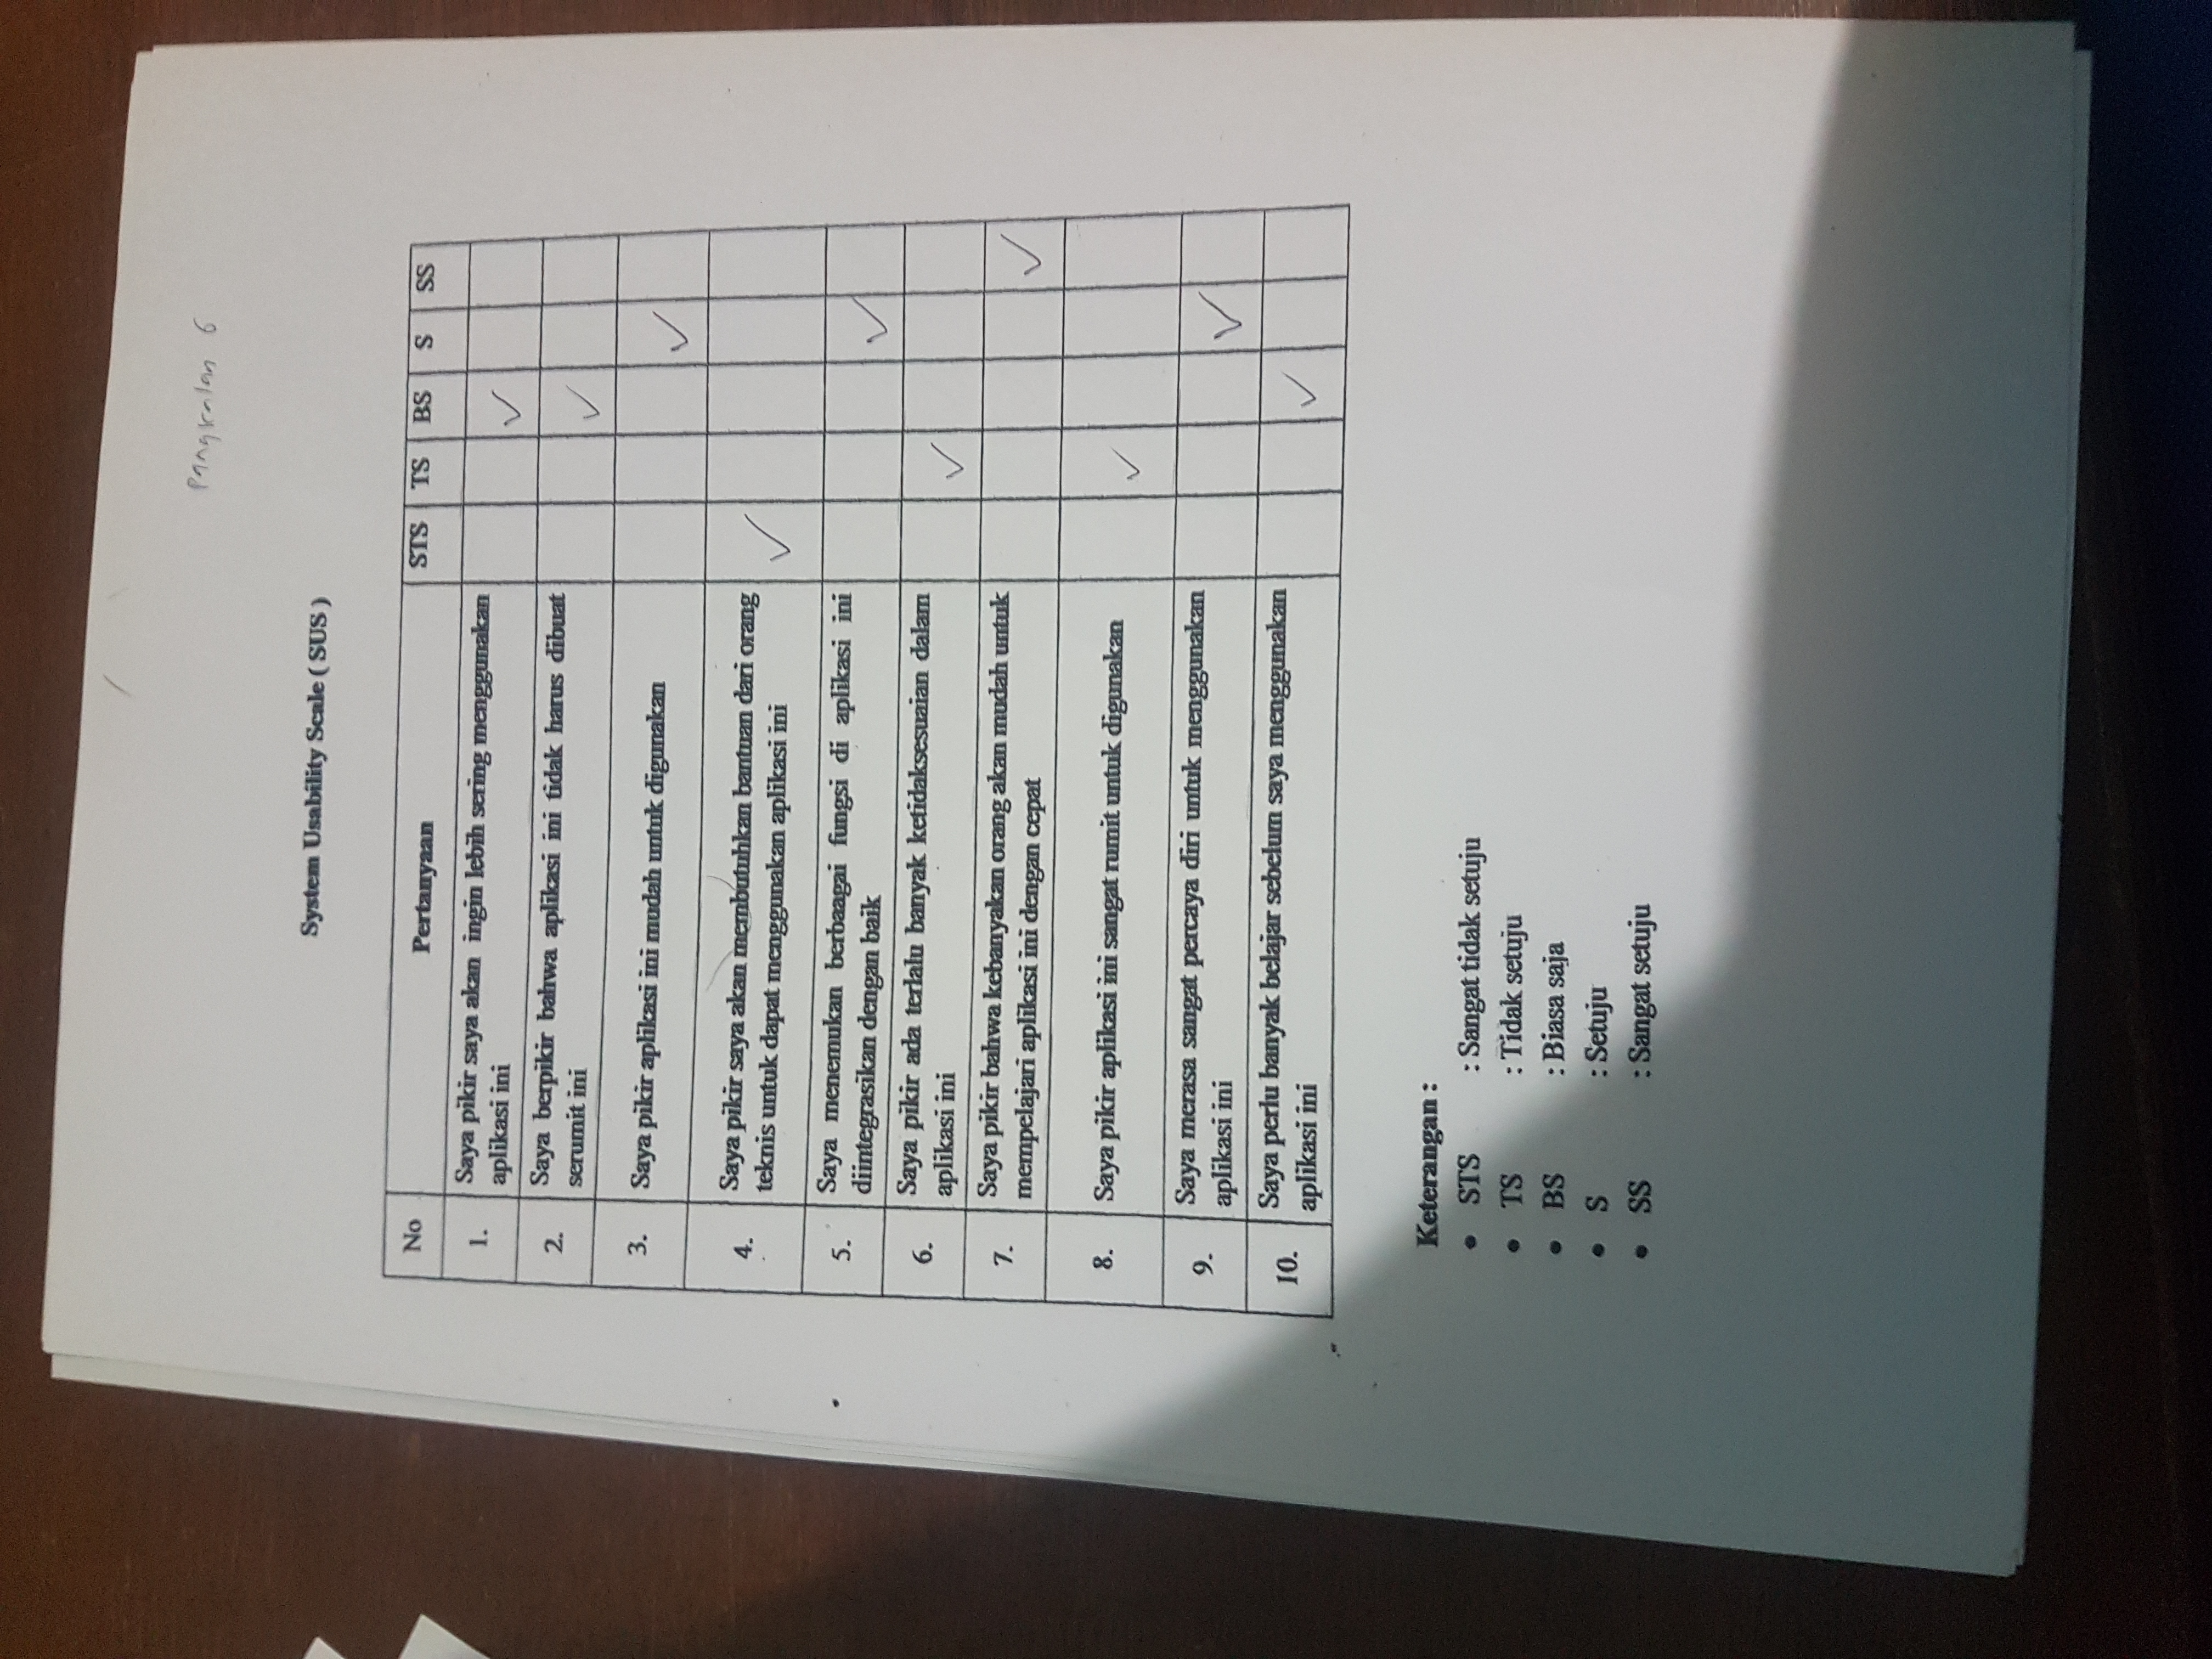
\includegraphics [width = 17cm,angle=-90]{gambar/pengujian/pangkalan6}
\end{figure}
\begin{figure}[H]
	\center
	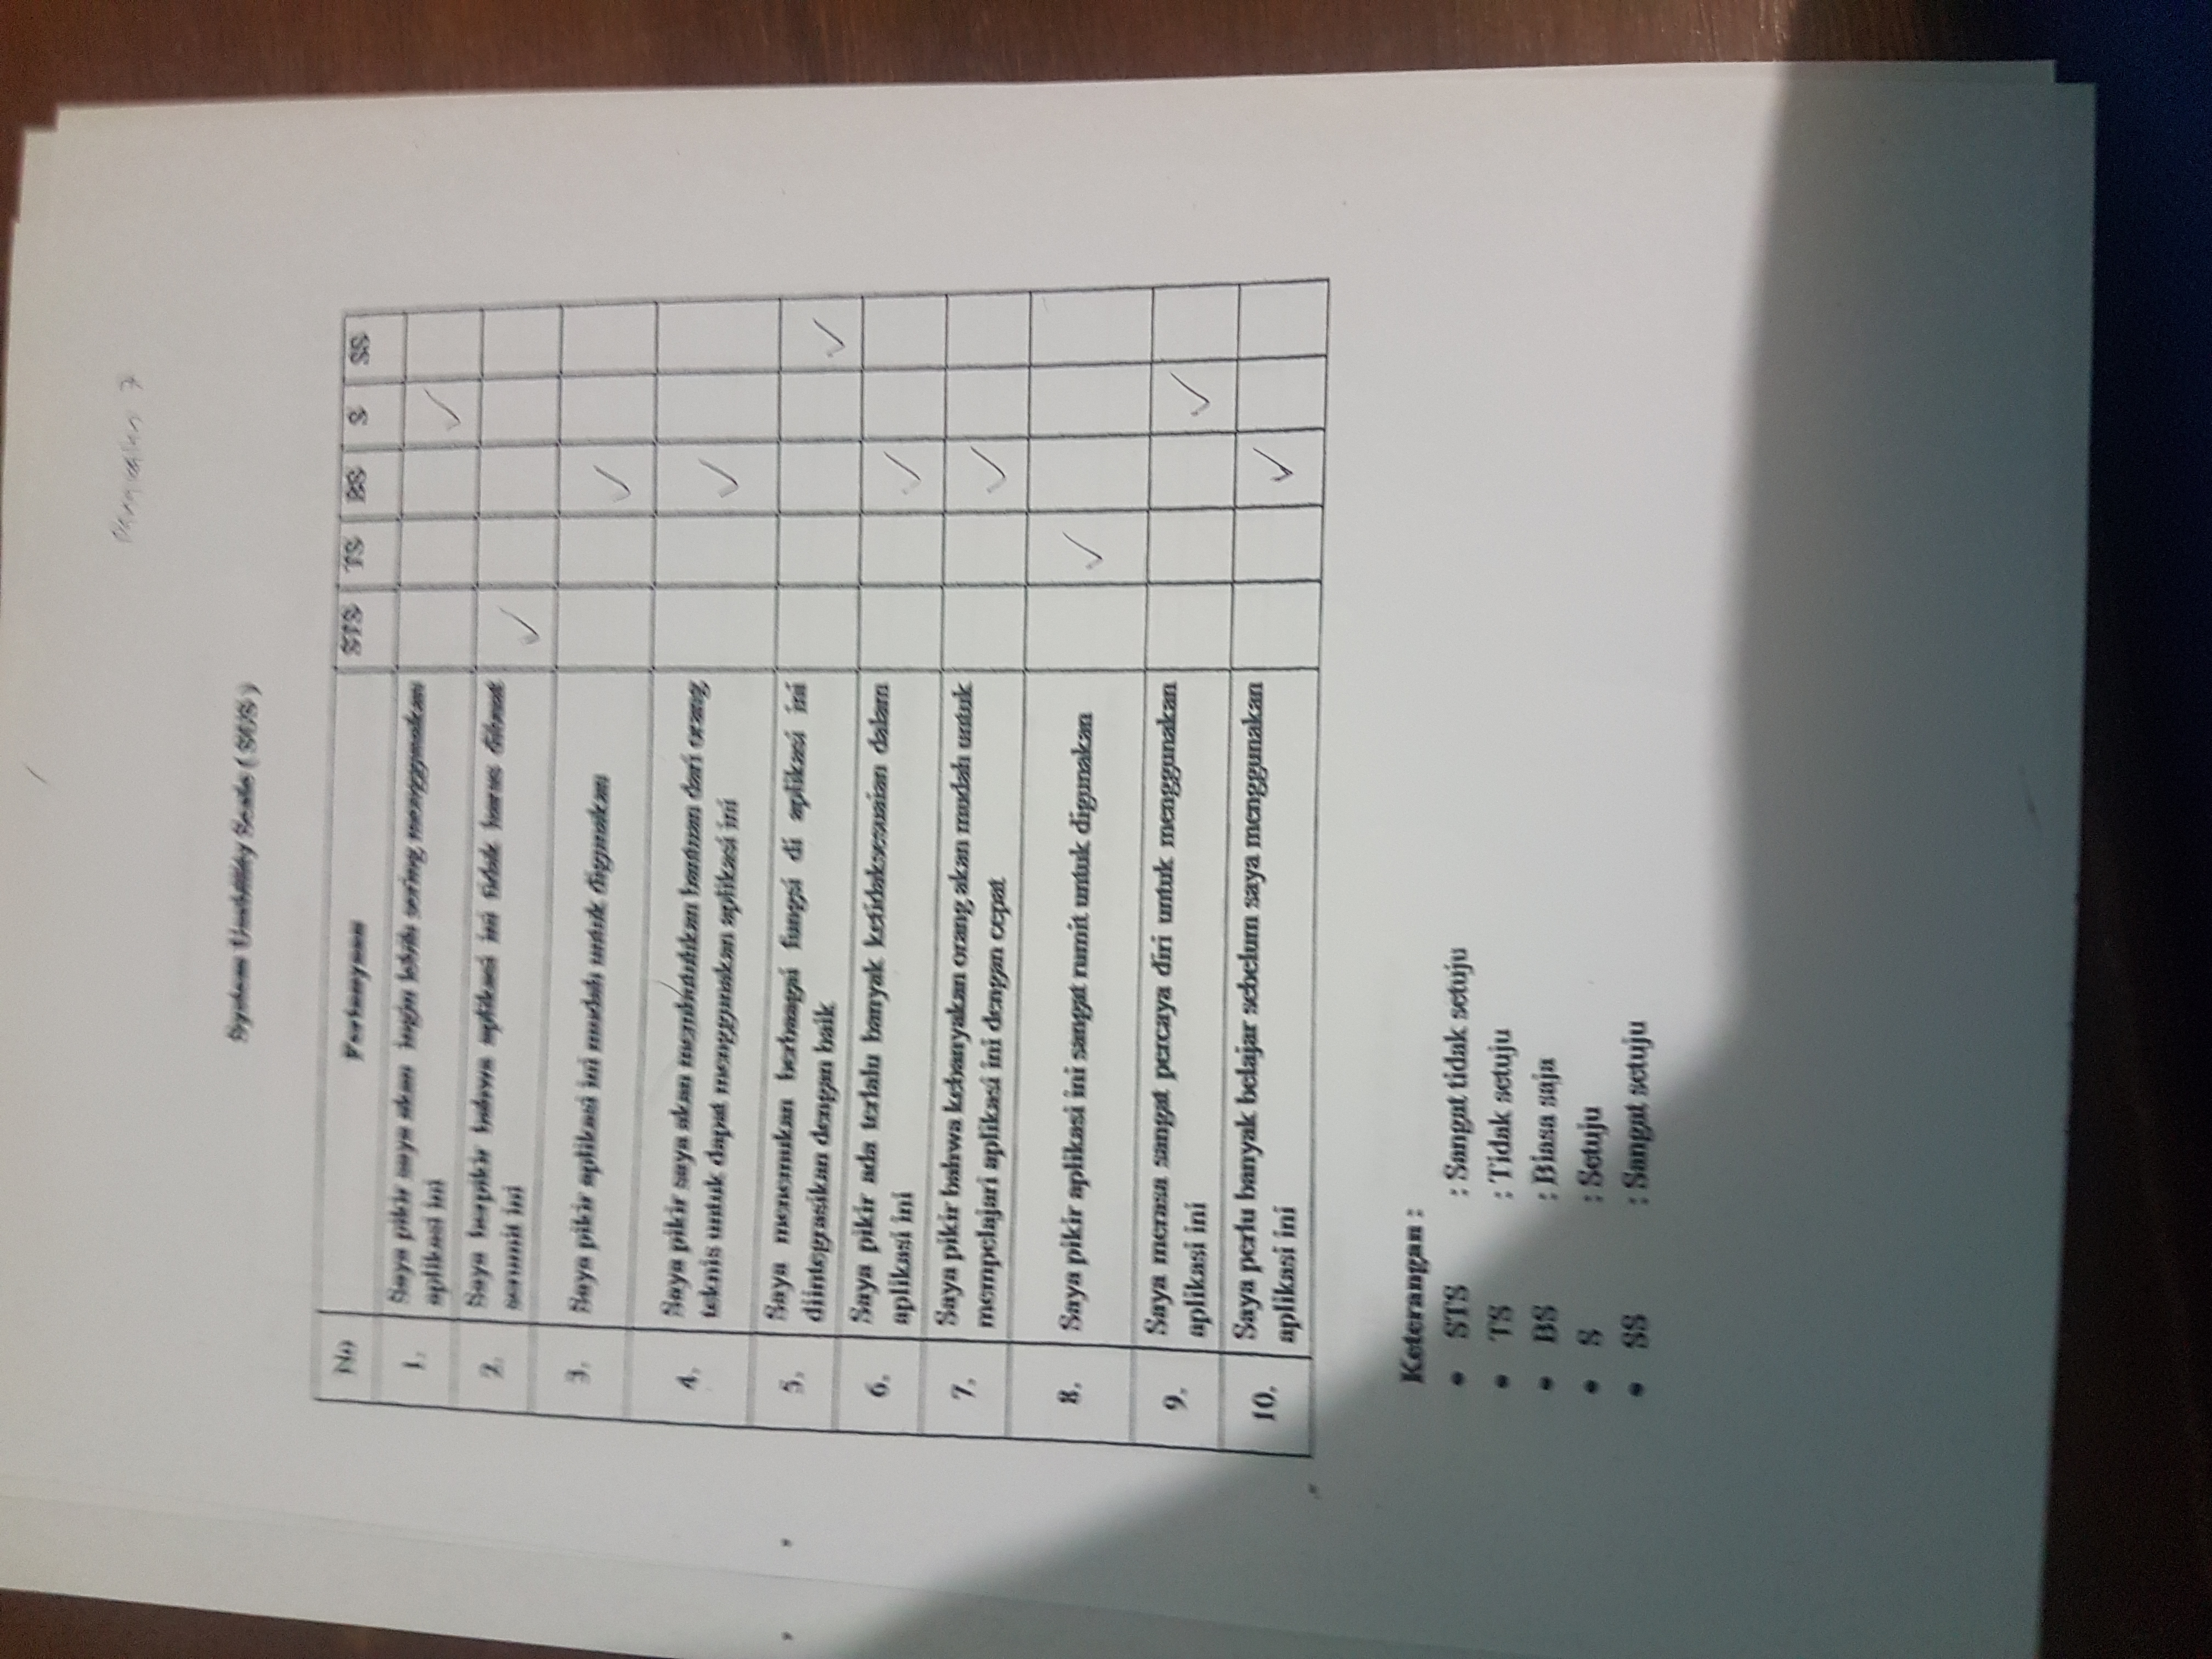
\includegraphics [width = 17cm,angle=-90]{gambar/pengujian/pangkalan7}
\end{figure}
\begin{figure}[H]
	\center
	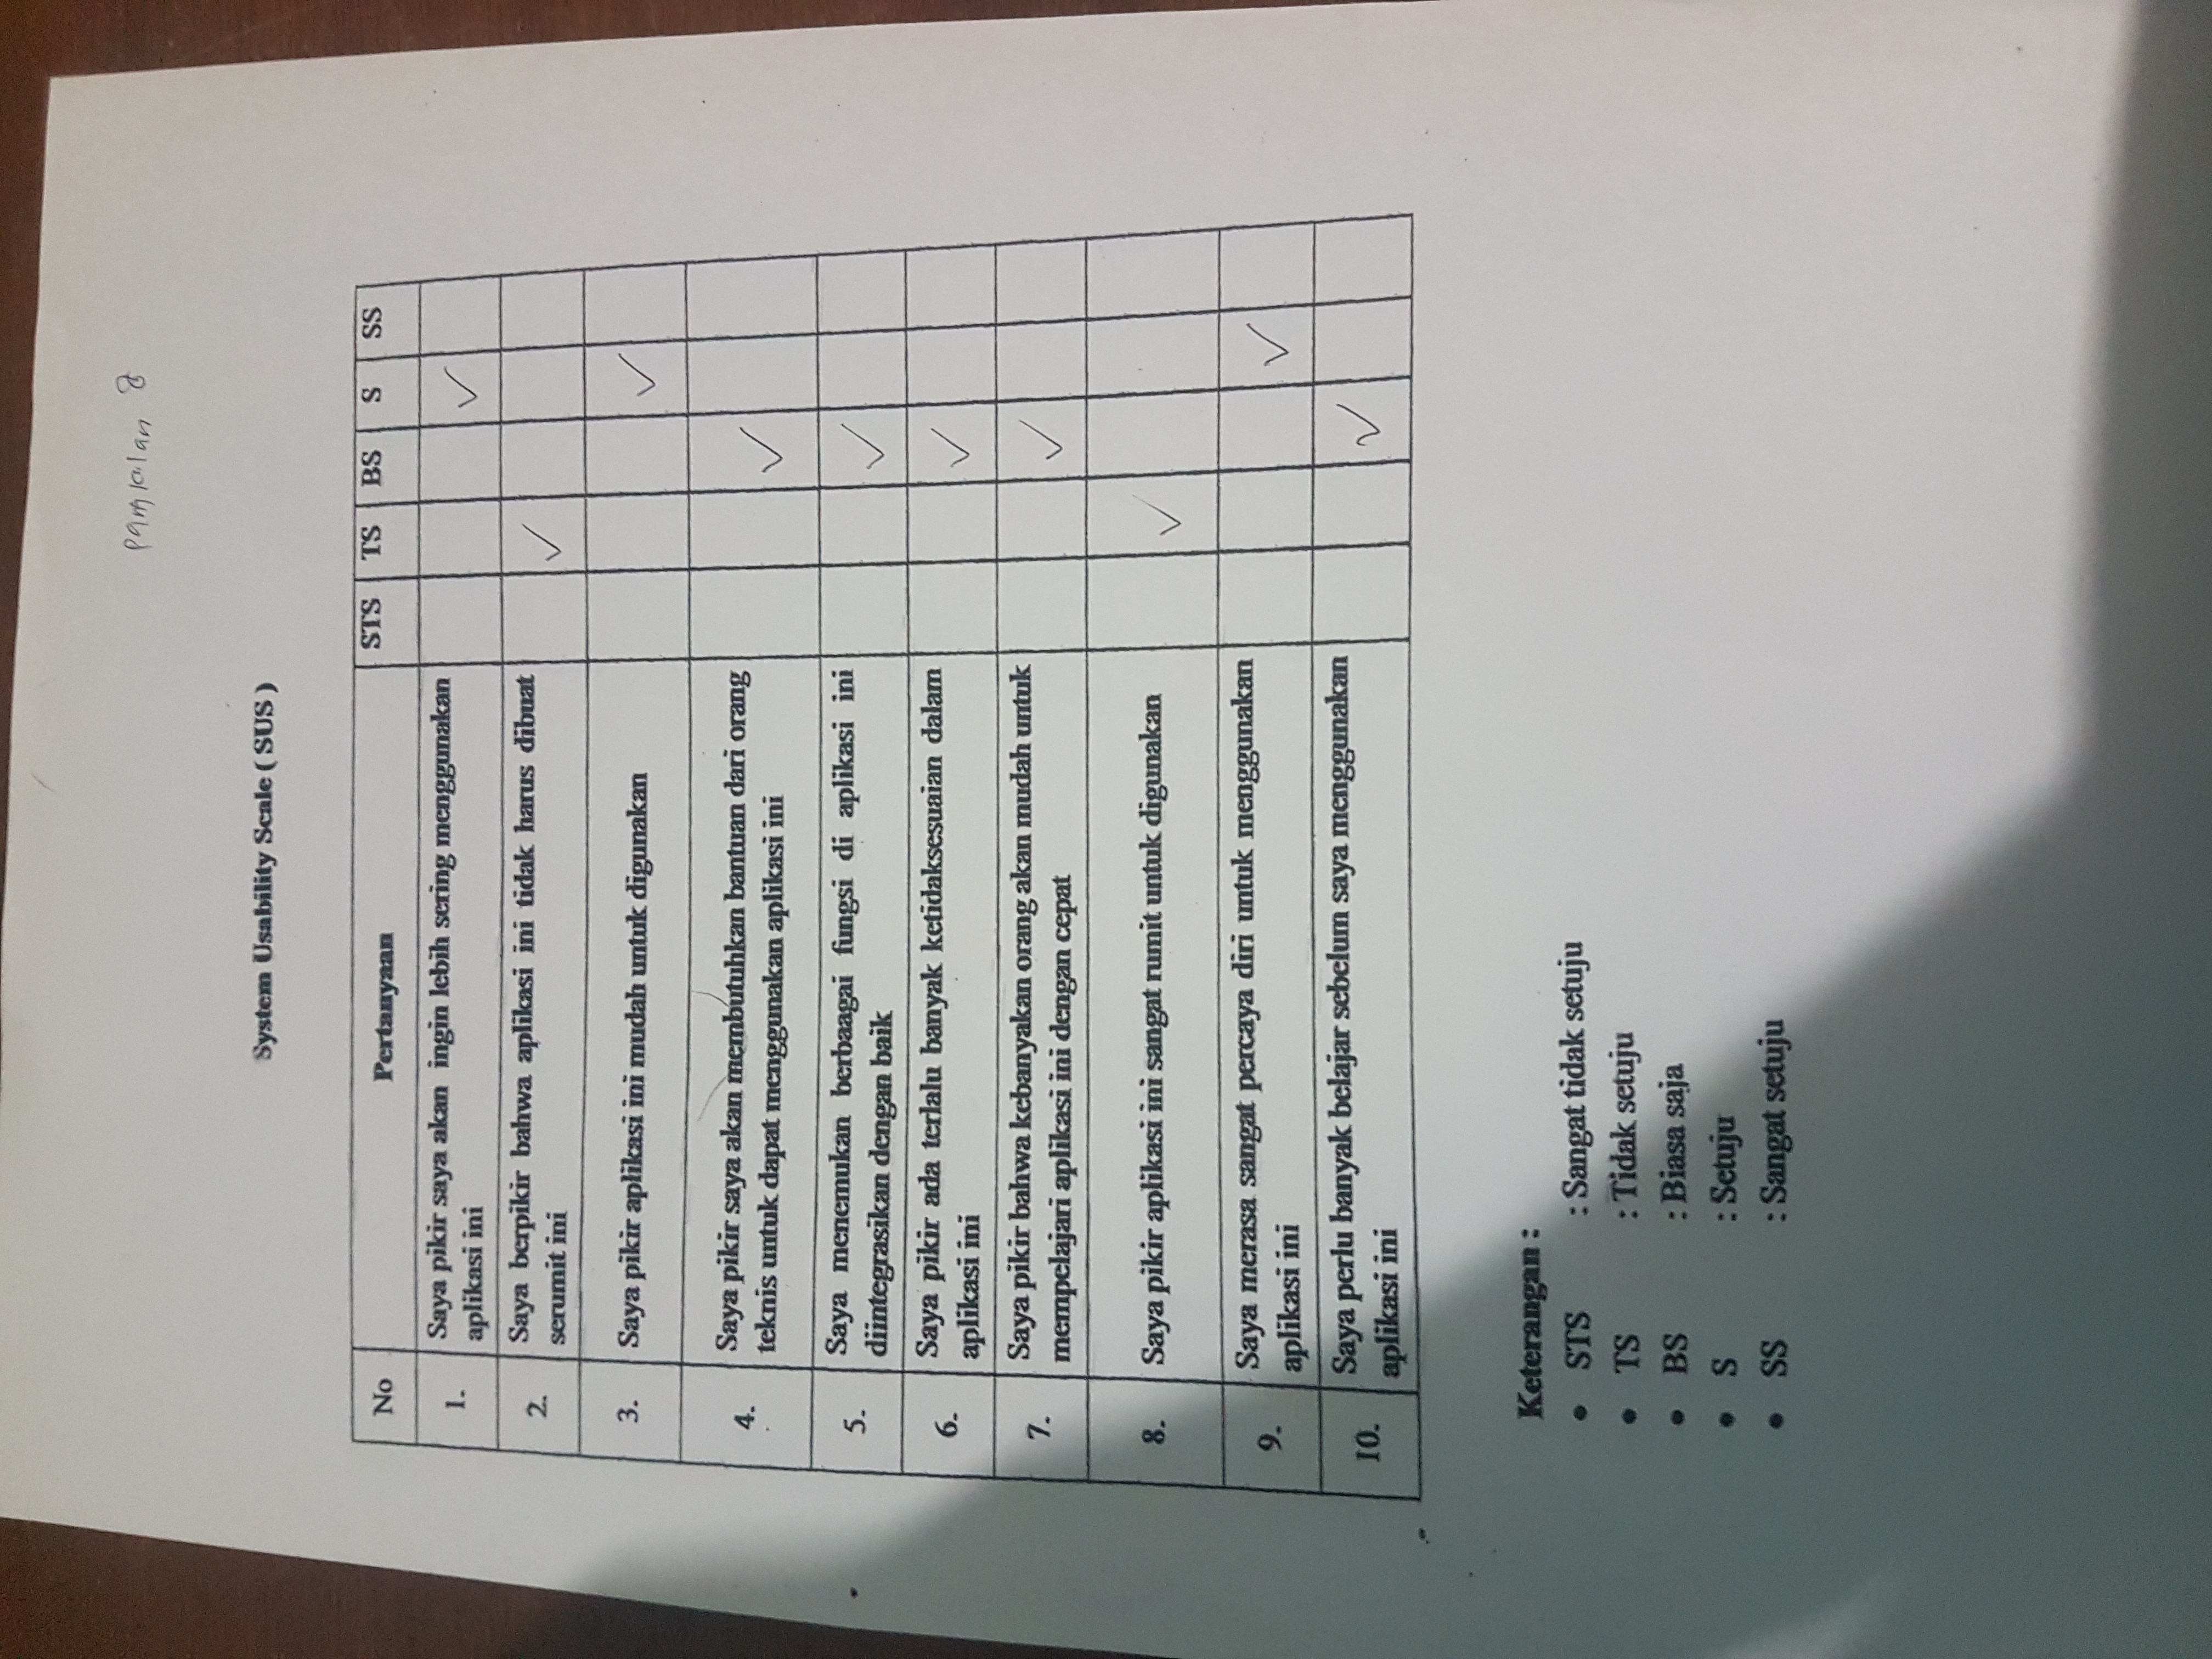
\includegraphics [width = 17cm,angle=-90]{gambar/pengujian/pangkalan8}
\end{figure}

%-----------------------------------------------------------------------------%
\addcontentsline{toc}{chapter}{LAMPIRAN 3}
\chapter*{Lampiran 3}
\newappendix{Lampiran 3. Foto Pengujian \textit{Usability}}

\begin{figure}[H]
	\includegraphics [width = 9cm]{gambar/pengujian/uji4}
	\includegraphics [width = 8cm]{gambar/pengujian/uji5}
\end{figure}

\begin{figure}[H]
	\includegraphics [width= 15cm]{gambar/pengujian/uji2}
\end{figure}

\begin{figure}[H]
	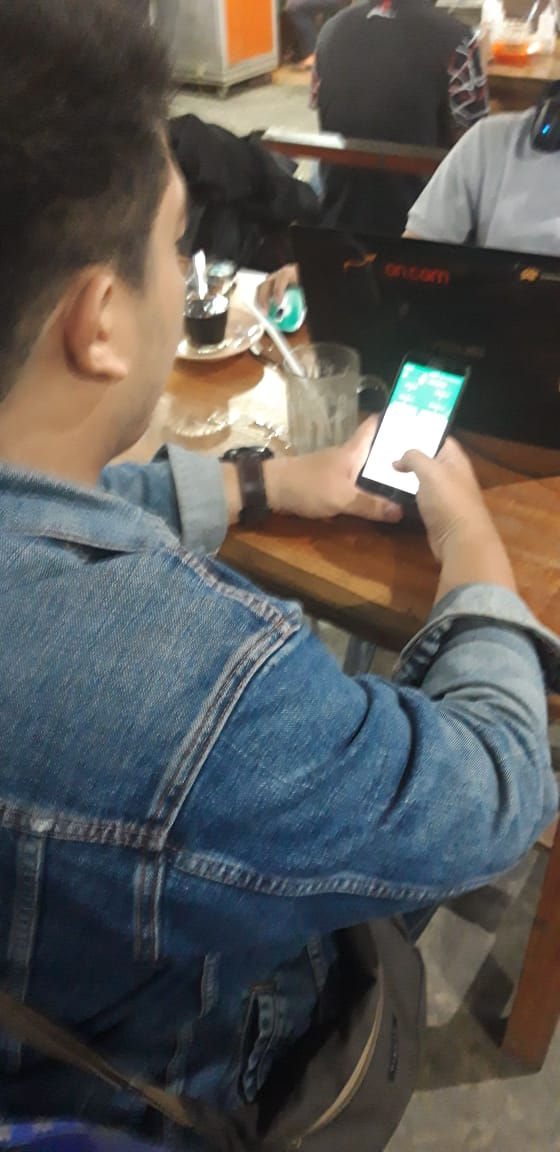
\includegraphics [height= 12cm]{gambar/pengujian/uji3}
	\includegraphics [height = 12cm]{gambar/pengujian/uji1}
\end{figure}
%-----------------------------------------------------------------------------%
\addcontentsline{toc}{chapter}{LAMPIRAN 4}
\chapter*{Lampiran 4}
\newappendix{Lampiran 4. Foto Wawancara Analisa Permasalahan dengan  \textit{User}}
\begin{figure}[H]
	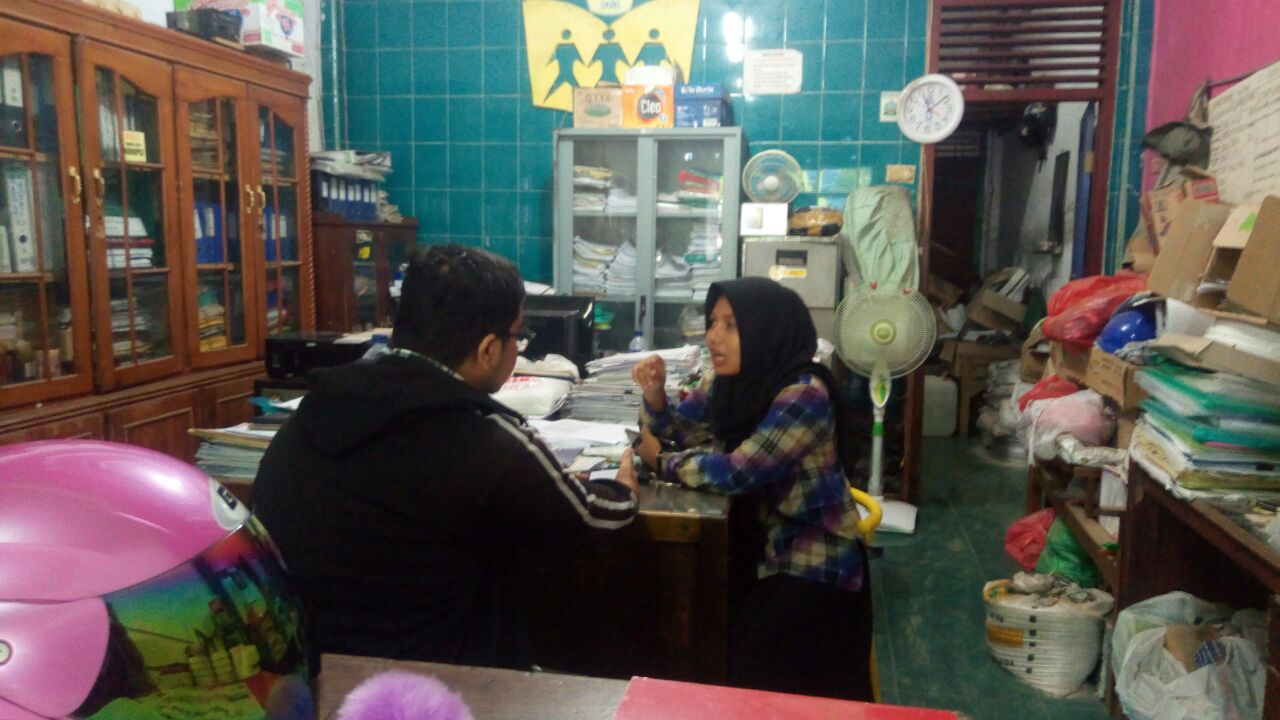
\includegraphics [width = 9cm]{gambar/wawancara/wawancara1}
	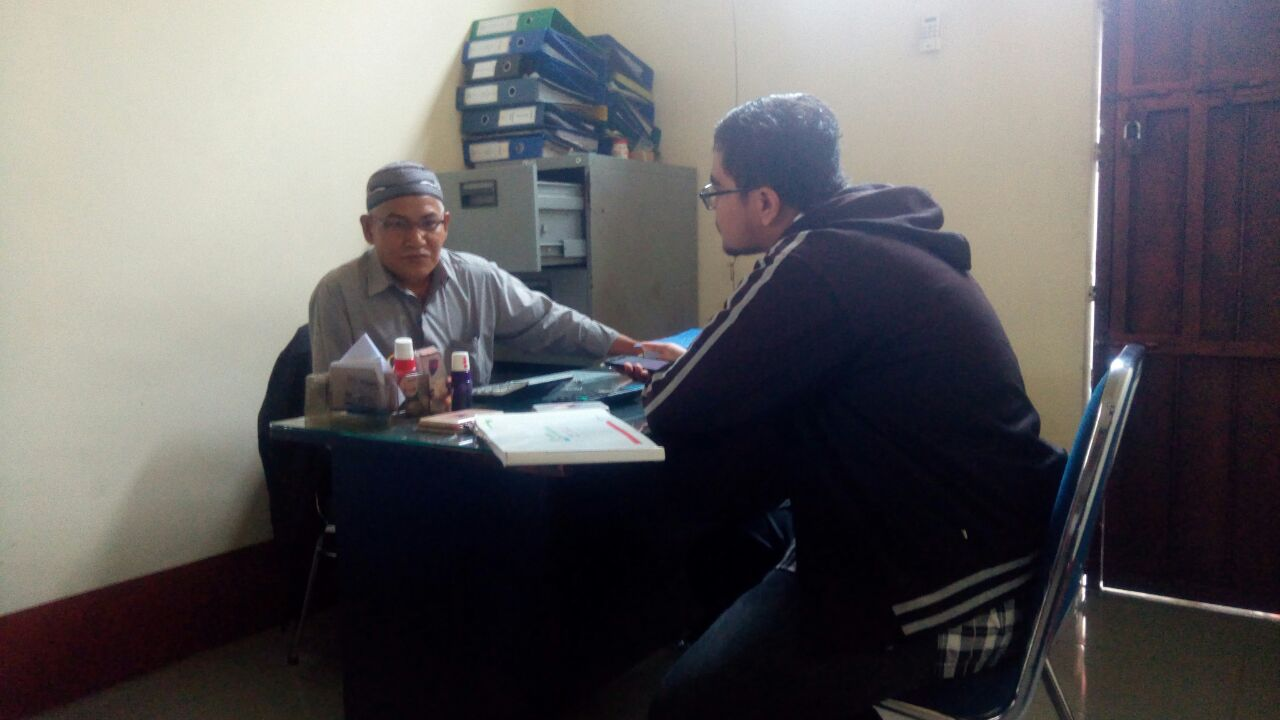
\includegraphics [width = 8cm]{gambar/wawancara/wawancara3}
\end{figure}

\begin{figure}[H]
	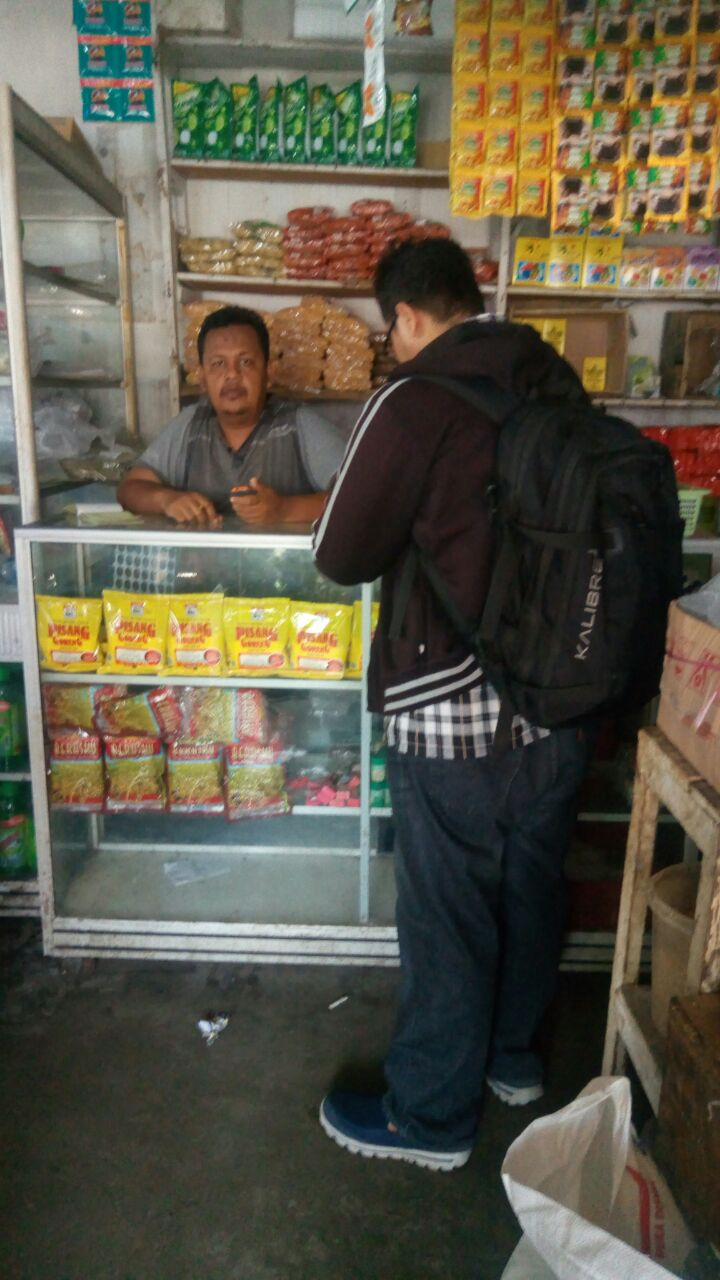
\includegraphics [height = 12cm]{gambar/wawancara/wawancara2}
	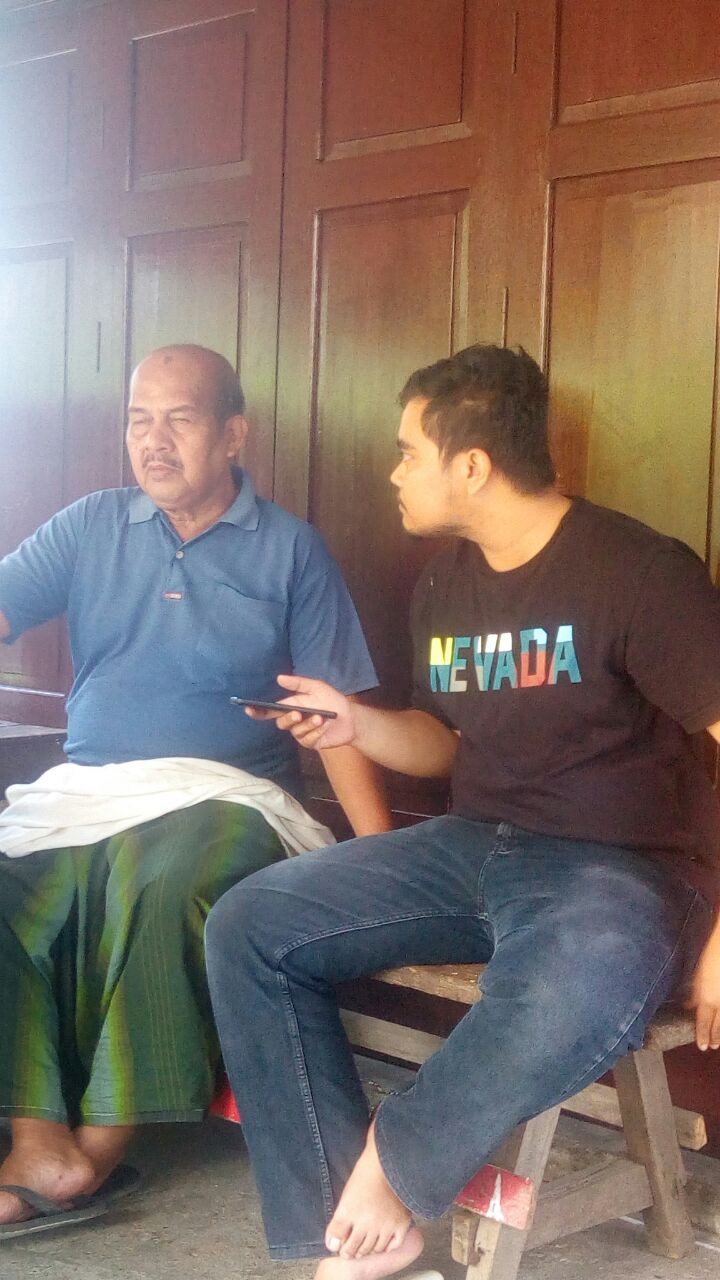
\includegraphics [height = 12cm]{gambar/wawancara/wawancara4}
\end{figure}


\begin{figure}[H]
	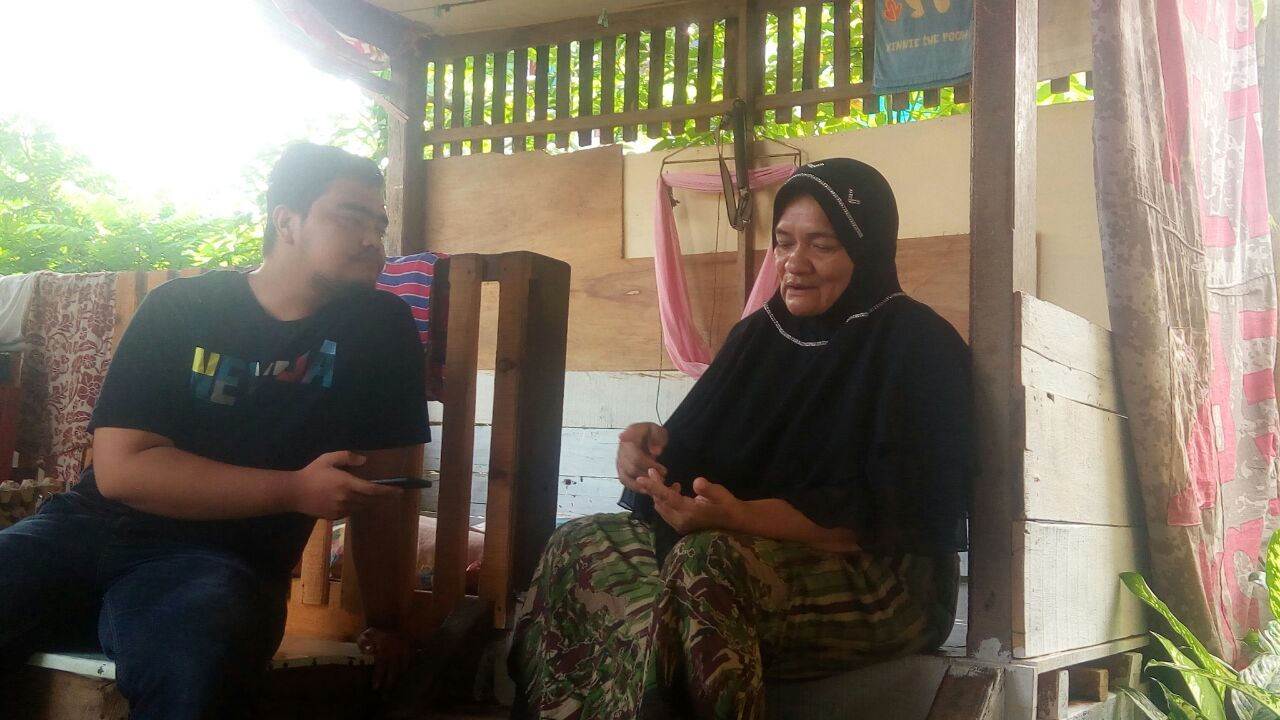
\includegraphics [width = 12cm]{gambar/wawancara/wawancara5}
	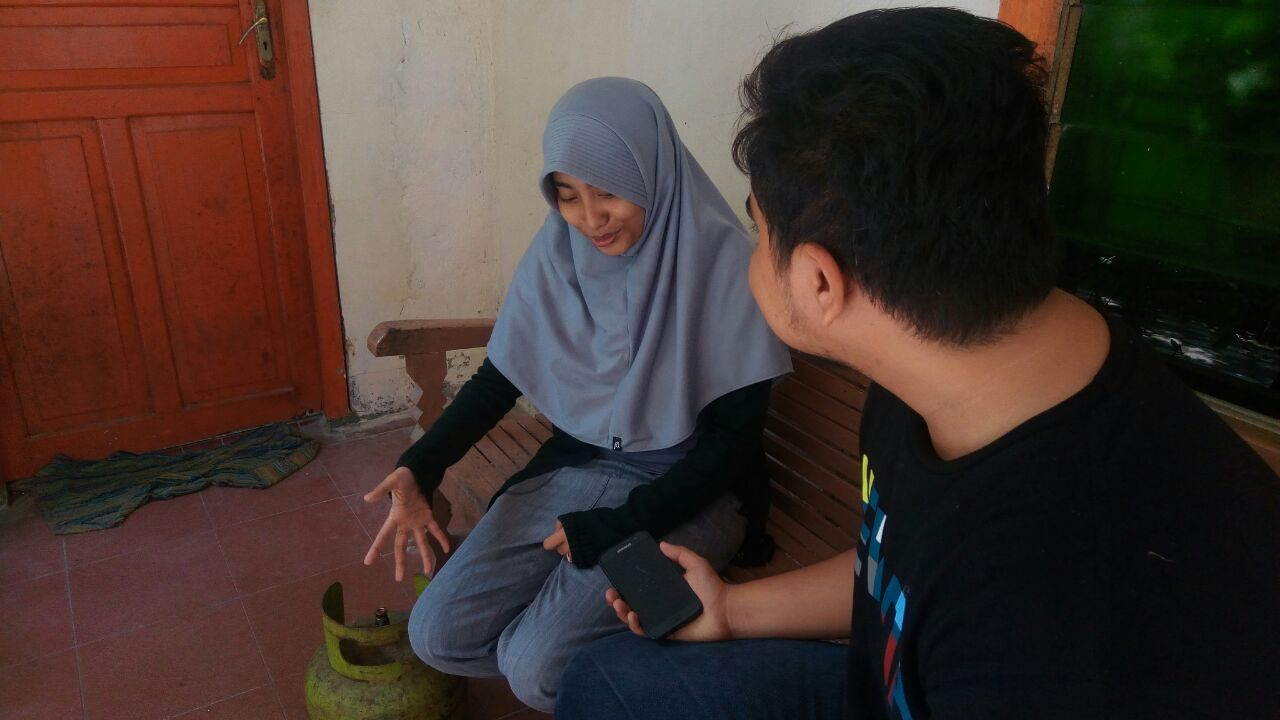
\includegraphics [width = 12cm]{gambar/wawancara/wawancara6}
\end{figure}

%-----------------------------------------------------------------------------%

%Lampiran 4 Laporan Usability

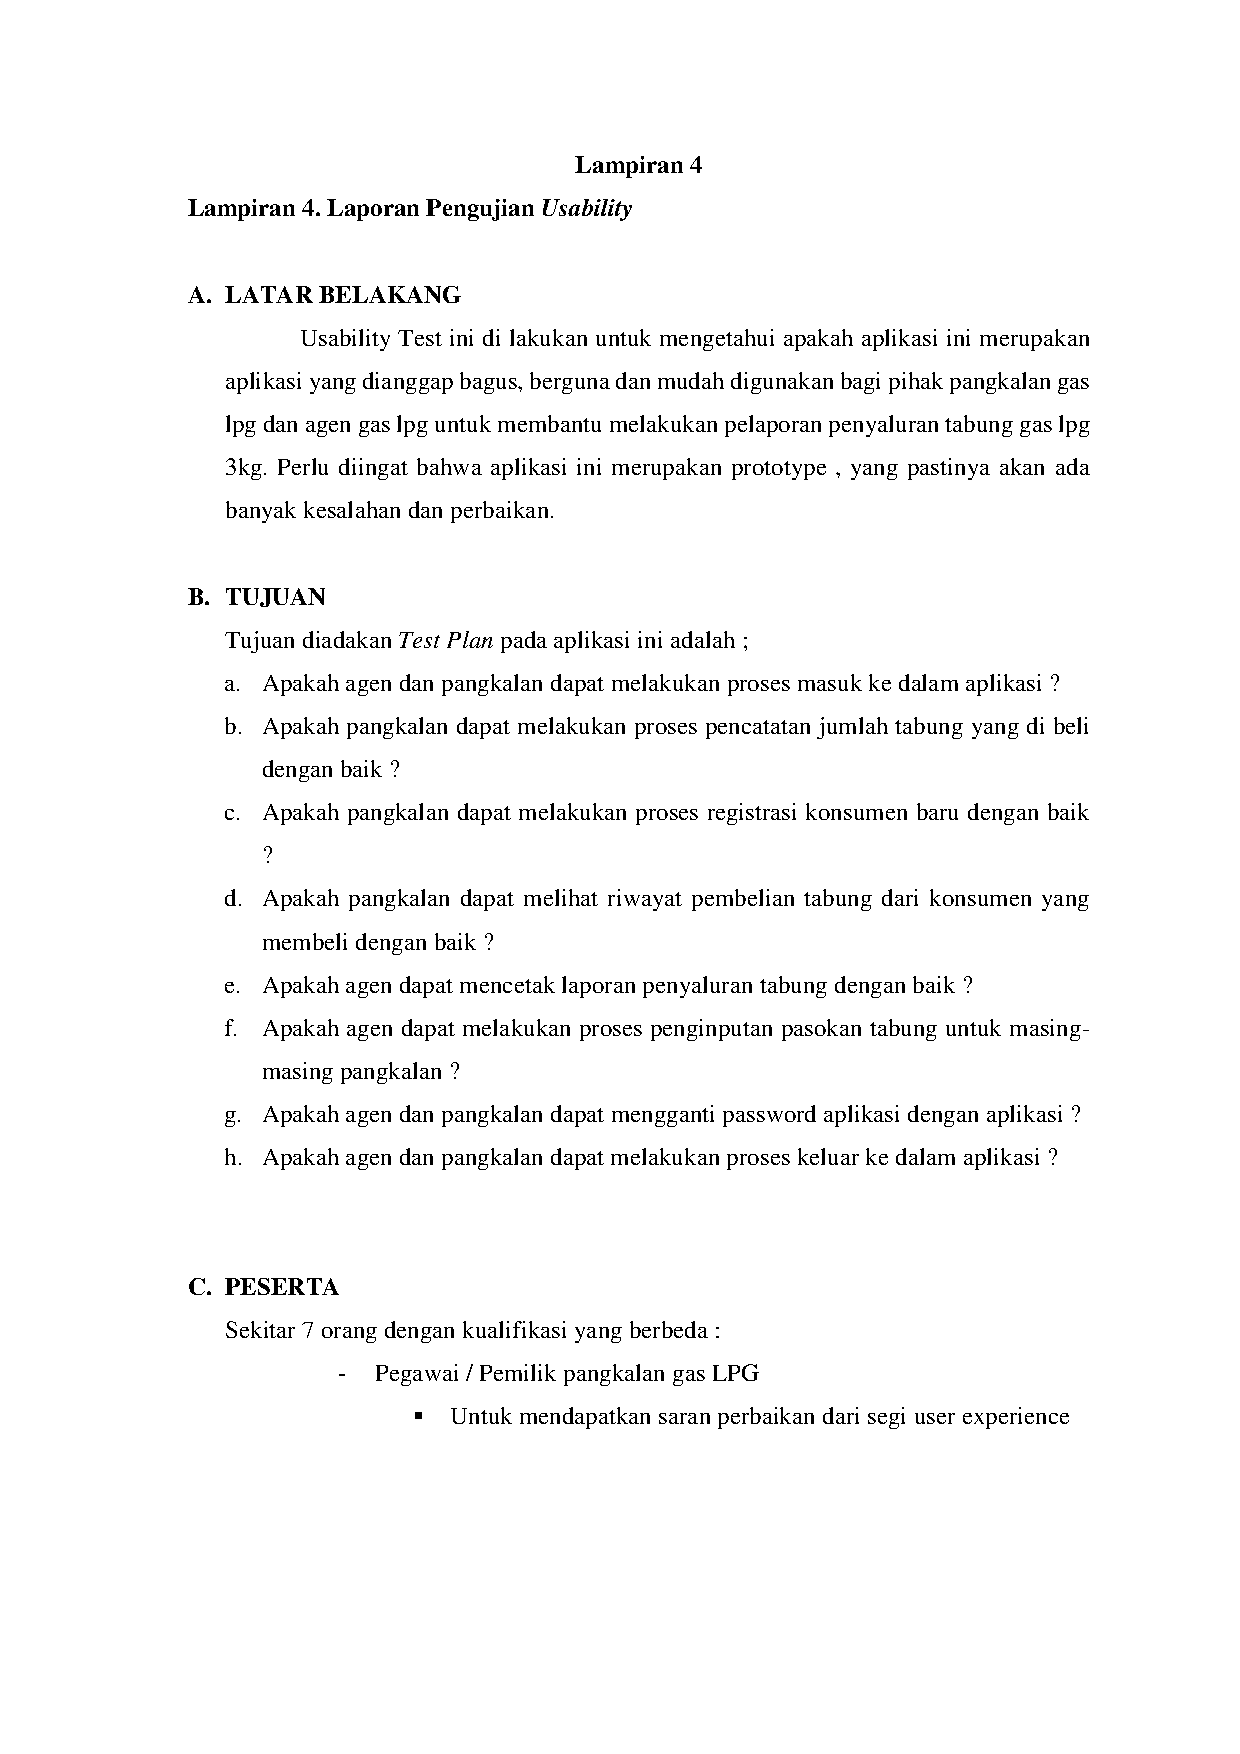
\includepdf[pages=1,scale=.8,pagecommand={
	\addcontentsline{toc}{chapter}{LAMPIRAN 5} 
	\chapter*{Lampiran 5}
	\newappendix{Lampiran 5. Laporan Hasil Pengujian \textit{Usability}}
},linktodoc=true]{laporan_usability}
\includepdf[pages=2-,scale=.8,pagecommand={},linktodoc=true]{laporan_usability}

%-----------------------------------------------------------------------------%
\addcontentsline{toc}{chapter}{LAMPIRAN 6}
\chapter*{Lampiran 6}
\newappendix{Lampiran 6. Contoh\textit{ Source Code} yang digunakan pada Sistem}

	\lstset{language=Java,
	basicstyle=\ttfamily\scriptsize\color{black},
	keywordstyle=\color{javapurple}\bfseries,
	stringstyle=\color{javared},
	commentstyle=\color{javagreen},
	morecomment=[s][\color{javadocblue}]{/**}{*/},
	numbers=left,
	numberstyle=\tiny\color{black},
	showstringspaces=false,
	numbersep=10pt,
	tabsize=4,
	showspaces=false,
	showstringspaces=false,
	autogobble=true,
	xleftmargin=2em
}

\begin{lstlisting}[caption=Potongan kode \textit{model} basis data layanan web, label=modelWebservice]
@Entity
public class Penerimaan {
public Penerimaan(Date tanggal, Integer jmlTabung, Ref<Laporan> laporan, 
Ref<Pangkalan> pangkalan, Boolean statusVerifikasi) {
setTanggal(tanggal);
setJmlTabung(jmlTabung);
setLaporan(laporan);
setPangkalan(pangkalan);
setStatusVerifikasi(statusVerifikasi);
}
}

\end{lstlisting}	


\begin{lstlisting}[caption=Potongan kode \textit{controller} layanan web, label=controllerWebservice]
public class PenerimaanAtur {

public Penerimaan baru(Date tanggal, Integer jmlTabung, Long idPangkalan) throws 
EntitasDuplikasiException, TidakDitemukanException, StokTidakCukupException {
Pangkalan pangkalan;


// Pastikan id pelanggan ada di entity penerimaan
try {
pangkalan = new PangkalanAtur().cari(idPangkalan);
} catch (TidakDitemukanException e) {
throw new 
TidakDitemukanException("Tidak ditemukan Pangkalan dengan id: '"+idPangkalan+"'");
}

// Pastikan penerimaan tidak memiliki tanggal dan pangkalan yang sama
try {
new PenerimaanAtur().cariTanggalPangkalan(tanggal, pangkalan);
throw new EntitasDuplikasiException("telah ada penjualan dengan tanggal :"+tanggal+"
dan pangkalan : "+pangkalan.getNamaPangkalan());
} catch (TidakDitemukanException e) {}


Ref<Pangkalan> refPangkalan = Ref.create(pangkalan);

//tambah penerimaan dengan refLaporan null
Penerimaan penerimaan = new Penerimaan(tanggal, jmlTabung, null, refPangkalan, false);
ofy().save().entity(penerimaan).now();


return penerimaan;
}


}

\end{lstlisting}

\begin{lstlisting}[caption=Potongan kode \textit{controller} layanan web, label=controllerWebservice]
public class PenerimaanAtur {

public Penerimaan baru(Date tanggal, Integer jmlTabung, Long idPangkalan) 
throws EntitasDuplikasiException, TidakDitemukanException, StokTidakCukupException {
Pangkalan pangkalan;

// Pastikan id pelanggan ada di entity penerimaan
try {
pangkalan = new PangkalanAtur().cari(idPangkalan);
} catch (TidakDitemukanException e) {
throw new TidakDitemukanException("Tidak ditemukan Pangkalan dengan id: '"+idPangkalan+"'");
}

// Pastikan penerimaan tidak memiliki tanggal dan pangkalan yang sama
try {
new PenerimaanAtur().cariTanggalPangkalan(tanggal, pangkalan);
throw new EntitasDuplikasiException("telah ada penjualan dengan tanggal :"+tanggal+"
dan pangkalan : "+pangkalan.getNamaPangkalan());
} catch (TidakDitemukanException e) {}

Ref<Pangkalan> refPangkalan = Ref.create(pangkalan);

//tambah penerimaan dengan refLaporan null
Penerimaan penerimaan = new Penerimaan(tanggal, jmlTabung, null, refPangkalan, false);
ofy().save().entity(penerimaan).now();
return penerimaan;
}
}

\end{lstlisting}	

\begin{lstlisting}[caption=Potongan kode API layanan web, label=apiWebservice]
@Api(name="penerimaan",
version="v1",
title = "Penerimaan",
description="API untuk Model Penerimaan. ",
apiKeyRequired=AnnotationBoolean.TRUE)
public class PenerimaanApi {
@ApiMethod(name = "daftar", httpMethod = HttpMethod.GET)
public List<PenerimaanJSON> daftar() {

List<Penerimaan> daftar = new PenerimaanAtur().daftar();
List<PenerimaanJSON> daftarJSON = new ArrayList<PenerimaanJSON>();

for(Penerimaan baris : daftar)
daftarJSON.add(new PenerimaanJSON(baris));

return daftarJSON;
}

@ApiMethod(name = "daftarByPangkalan", httpMethod = HttpMethod.POST)
public List<PenerimaanJSON> daftarByPangkalan(DaftarByPangkalanJSON params) 
throws TidakDitemukanException {
Pangkalan pangkalan = new PangkalanAtur().cari(params.idPangkalan);
List<Penerimaan> daftar = new PenerimaanAtur().daftarByPangkalan(pangkalan);
List<PenerimaanJSON> daftarJSON = new ArrayList<PenerimaanJSON>();

for(Penerimaan baris : daftar) {
daftarJSON.add(new PenerimaanJSON(baris));
}

return daftarJSON;
}

}

\end{lstlisting}

	\lstset{language=Java,
	basicstyle=\ttfamily\scriptsize\color{black},
	keywordstyle=\color{javapurple}\bfseries,
	stringstyle=\color{javared},
	commentstyle=\color{javagreen},
	morecomment=[s][\color{javadocblue}]{/**}{*/},
	numbers=left,
	numberstyle=\tiny\color{black},
	showstringspaces=false,
	numbersep=10pt,
	tabsize=4,
	showspaces=false,
	showstringspaces=false,
	autogobble=true,
	xleftmargin=2em
}

\begin{lstlisting}[caption=Potongan kode \textit{model} aplikasi berbasis web, label=modelWeb]
public class PangkalanService extends AppService{

private static final String baseUrl=AppService.getWebService();

public ListPangkalanJson getPangkalan()
{
String restUrl = baseUrl+"/pangkalan/v1/daftar";

String jsonString = getJsonString(restUrl);
ListPangkalanJson jsonObject = null;

//Konversi json string ke class object
try{
Gson gson = new GsonBuilder().create();
jsonObject = gson.fromJson(jsonString, ListPangkalanJson.class);            
}
catch(JsonSyntaxException ex)
{
ex.printStackTrace();
}

return jsonObject;
}

}

\end{lstlisting}

\lstset{language=HTML,
	basicstyle=\ttfamily\scriptsize\color{black},
	keywordstyle=\color{javapurple}\bfseries,
	stringstyle=\color{javared},
	commentstyle=\color{javagreen},
	morecomment=[s][\color{javadocblue}]{/**}{*/},
	numbers=left,
	numberstyle=\tiny\color{black},
	showstringspaces=false,
	numbersep=10pt,
	tabsize=4,
	showspaces=false,
	showstringspaces=false,
	autogobble=true,
	xleftmargin=2em
}
\begin{lstlisting}[caption=Potongan kode \textit{view} aplikasi berbasis web, label=viewWeb]
<%@ taglib prefix="c" uri="http://java.sun.com/jsp/jstl/core" %>
<!-- Main content -->
<section class="content">
<!-- Small boxes (Stat box) -->
<div class="row">
<c:choose>
<c:when test="${sessionScope.userGroup == 'administrator'}">
<div class="col-lg-6 col-xs-6">
<!-- small box -->
<div class="small-box bg-aqua">
<div class="inner">
<h3>${jmlAgen}</h3>
<p>Jumlah Agen</p>
</div>
<div class="icon">
<i class="fa fa-user"></i>
</div>
<a href="#" class="small-box-footer">More info 
<i class="fa fa-arrow-circle-right"></i></a>
</div>
</div><!-- ./col -->

\end{lstlisting}


\lstset{language=Java,
	basicstyle=\ttfamily\scriptsize\color{black},
	keywordstyle=\color{javapurple}\bfseries,
	stringstyle=\color{javared},
	commentstyle=\color{javagreen},
	morecomment=[s][\color{javadocblue}]{/**}{*/},
	numbers=left,
	numberstyle=\tiny\color{black},
	showstringspaces=false,
	numbersep=10pt,
	tabsize=4,
	showspaces=false,
	showstringspaces=false,
	autogobble=true,
	xleftmargin=2em
}
\begin{lstlisting}[caption=Potongan kode \textit{controller} aplikasi berbasis web, label=controllerWeb]
@SuppressWarnings("serial")
@WebServlet(
name="Dashboard",
urlPatterns={"/dashboard"}, 
description="Halaman Dashboard (admin)"
)
public class Dashboard extends HttpServlet{


@Override
protected void doGet(HttpServletRequest req, HttpServletResponse resp) 
throws ServletException, IOException {

HttpSession session = req.getSession();
//cek otentikasi user dengan session
if (session == null || session.getAttribute("userMail") == null) {
resp.sendRedirect(AppService.getBaseUrl(req)+"/login");
return;
}

List<AgenJson> agenJsons;
List<PangkalanJson> pangkalanJsons;


if(session.getAttribute("userGroup").toString().compareTo("agen") == 0) {
Long idAgen =  (Long) session.getAttribute("userIdAgen");

pangkalanJsons = new PangkalanService().getPangkalanByAgen(idAgen).getItems();

req.setAttribute("baseUrl", AppService.getBaseUrl(req));
req.setAttribute("pageTitle", "Dashboard");
req.setAttribute("webserviceUrl", AppService.getWebService());
req.setAttribute("content", "Home");

req.setAttribute("jmlPangkalan", pangkalanJsons.size());


resp.setContentType("text/html");
RequestDispatcher jsp = req.getRequestDispatcher(KonstantaWebApp.JSP_FOLDER+"Dashboard.jsp");
jsp.forward(req, resp);
}


}

\end{lstlisting}

	\lstset{language=HTML,
	basicstyle=\ttfamily\scriptsize\color{black},
	keywordstyle=\color{javapurple}\bfseries,
	stringstyle=\color{javared},
	commentstyle=\color{javagreen},
	morecomment=[s][\color{javadocblue}]{/**}{*/},
	numbers=left,
	numberstyle=\tiny\color{black},
	showstringspaces=false,
	numbersep=10pt,
	tabsize=4,
	showspaces=false,
	showstringspaces=false,
	autogobble=true,
	xleftmargin=2em
}

\begin{lstlisting}[caption=Potongan kode Login memakai email aplikasi berbasis web, label=loginWeb]
<script src="assets/modules/bootstrap/js/bootstrap.min.js"></script>
<script type="text/javascript">
var BASE_URL = '${baseUrl}';
$(document).ready(function(){
$('[data-toggle="tooltip"]').tooltip();
});
</script>

\end{lstlisting}

\lstset{language=Java,
	basicstyle=\ttfamily\scriptsize\color{black},
	keywordstyle=\color{javapurple}\bfseries,
	stringstyle=\color{javared},
	commentstyle=\color{javagreen},
	morecomment=[s][\color{javadocblue}]{/**}{*/},
	numbers=left,
	numberstyle=\tiny\color{black},
	showstringspaces=false,
	numbersep=10pt,
	tabsize=4,
	showspaces=false,
	showstringspaces=false,
	autogobble=true,
	xleftmargin=2em
}
\begin{lstlisting}[caption=Potongan kode ekspor data aplikasi berbasis web, label=eksporWeb]
protected void generatePdf(Document doc, String[] periode, EksporPelaporanJson data) 
throws IOException {
doc.add(new Paragraph("Data Laporan Penyaluran Gas 3Kg" ).setBold()
.setFontSize(14).setTextAlignment(TextAlignment.CENTER));
Table detailPangkalan = new Table(3);
detailPangkalan.setMarginTop(18);
detailPangkalan.setMarginLeft(8);

detailPangkalan.addCell(new Cell().add(new Paragraph("Nama Pangkalan"))
.setBorder(Border.NO_BORDER));
detailPangkalan.addCell(new Cell().add(new Paragraph(":")).setBorder(Border.NO_BORDER));
detailPangkalan.addCell(new Cell().add(new Paragraph(data.getNamaPangkalan()))
.setBorder(Border.NO_BORDER));

doc.add(detailPangkalan);
doc.add(generateTable(periode, data.getPelaporan()));
}
\end{lstlisting}

\lstset{language=HTML,
	basicstyle=\ttfamily\scriptsize\color{black},
	keywordstyle=\color{javapurple}\bfseries,
	stringstyle=\color{javared},
	commentstyle=\color{javagreen},
	morecomment=[s][\color{javadocblue}]{/**}{*/},
	numbers=left,
	numberstyle=\tiny\color{black},
	showstringspaces=false,
	numbersep=10pt,
	tabsize=4,
	showspaces=false,
	showstringspaces=false,
	autogobble=true,
	xleftmargin=2em
}

\begin{lstlisting}[caption=Potongan kode \textit{model} aplikasi berbasis android, label=modelMobile]
export class RestService {
apiUrl = 'https://gasapp-2018.appspot.com/_ah/api';

constructor(public http: HttpClient) {
console.log('Hello RestProvider Provider');
}

userAuthentication(phoneNumber) {
return new Promise((resolve, reject) => {
let headers = new HttpHeaders()
let data = {noHp:phoneNumber};
this.http.post(this.apiUrl+'/pangkalan/v1/auth', JSON.stringify(data), {headers: headers})
.subscribe(res => {
resolve(res);
}, (err) => {
reject(err);
});
});
}

}

\end{lstlisting}

\begin{lstlisting}[caption=Potongan kode \textit{view} aplikasi berbasis android, label=viewMobile]
<ion-header translucent="true">
<ion-toolbar id="toolbar-home" style="padding-top:0">
<ion-title>
<ion-img [src]="logo" class="logo"></ion-img>
</ion-title>
<ion-buttons slot="start">
<ion-menu-button autoHide="false"></ion-menu-button>
</ion-buttons>
</ion-toolbar>
</ion-header>

<ion-content fullscreen ion-padding color="light">

<!-- <ion-slides pager=true [options]="slideOptions"> 
<ion-slide *ngFor="let slide of slides">
<ion-img [src]="slide" class="slide-image"></ion-img>
</ion-slide> 
</ion-slides> -->
<div class="wrap-cover parallax-obj">
<div class="bg-profile shadow-3">
<ion-row class="panel-stats">
<ion-col id="stok" size="6">
<ion-text color="light" class="stats">
<h4>Stok Tabung</h4>
<p>{{statistik.stokTabung}}</p>
</ion-text> 
</ion-col>
</div>
</div>

\end{lstlisting}

\begin{lstlisting}[caption=Potongan kode \textit{controller} aplikasi berbasis android, label=controllerMobile]
export class HomePage {
logo = 'assets/img/logoPutih.png';

constructor(
private route:ActivatedRoute,
private custom:CustomService,
private menu: MenuController,
private storage: Storage,
private restService: RestService
) {
if(this.route.snapshot.paramMap.has('flashdata')){
this.custom.showAlert("", this.route.snapshot.paramMap.get('flashdata'));
}

this.storage.get("userData").then(res => {
this.userData = res;

this.restService.statistikTabung(this.userData.idPangkalan).then(res => {
let data:any = res;
this.statistik.stokTabung = data.stokTabung;
this.statistik.hariIni = data.tabungTerjualHariIni;
this.statistik.bulanIni = data.tabungTerjualBulanIni;
this.statistik.tahunIni = data.tabungTerjualTahunIni;
})
console.log(this.userData);
this.menu.enable(true, 'menu');
this.menu.open('menu');

}).catch(err => {
console.log(err);
});

}

}

\end{lstlisting}

	\lstset{language=Java,
	basicstyle=\ttfamily\scriptsize\color{black},
	keywordstyle=\color{javapurple}\bfseries,
	stringstyle=\color{javared},
	commentstyle=\color{javagreen},
	morecomment=[s][\color{javadocblue}]{/**}{*/},
	numbers=left,
	numberstyle=\tiny\color{black},
	showstringspaces=false,
	numbersep=10pt,
	tabsize=4,
	showspaces=false,
	showstringspaces=false,
	autogobble=true,
	xleftmargin=2em
}

\begin{lstlisting}[caption=Potongan kode Pengujian JUnit dengan kasus berhasil (\textit{test success}), label=testSuccess]
//cek tambah penerimaan
@Test
public void baru() throws EntitasDuplikasiException,
TidakDitemukanException, StokTidakCukupException {
Agen agen = this.buatAgen();
Pangkalan pangkalan = this.buatPangkalan(agen);

Penerimaan penerimaan = new PenerimaanAtur().baru(tanggalPenerimaan1, jmlTabungPenerimaan1, 
pangkalan.getId());
assertNotNull(penerimaan);
assertNotNull(penerimaan.getId());
assertNotNull(penerimaan.getKey());
assertNotNull(penerimaan.getTanggal());
assertEquals(penerimaan.getTanggal().compareTo(tanggalPenerimaan1), 0);
assertNotNull(penerimaan.getJmlTabung());
assertEquals(penerimaan.getJmlTabung().compareTo(jmlTabungPenerimaan1), 0);
assertNotNull(penerimaan.getPangkalan());
assertEquals(penerimaan.getPangkalan().compareTo(Ref.create(pangkalan)), 0);
assertNull(penerimaan.getLaporan());
assertNotNull(penerimaan.getStatusVerifikasi());
assertEquals(penerimaan.getStatusVerifikasi().compareTo(false), 0);
}
\end{lstlisting}

\begin{lstlisting}[caption=Potongan kode Pengujian JUnit dengan kasus gagal (\textit{test fail}), label=testFail]
//cek tambah penerimaan dengan tanggal null
@Test(expected = NullPointerException.class)
public void baruTanggalNull() throws EntitasDuplikasiException, TidakDitemukanException,
 StokTidakCukupException {
Agen agen = this.buatAgen();
Pangkalan pangkalan = this.buatPangkalan(agen);

new PenerimaanAtur().baru(null, jmlTabungPenerimaan1, pangkalan.getId());
}
\end{lstlisting}
%-----------------------------------------------------------------------------%
\addcontentsline{toc}{chapter}{LAMPIRAN 7}
\chapter*{Lampiran 7}
\newappendix{Lampiran 7. Class Diagram pada Database Sistem}
\begin{figure}[H]
	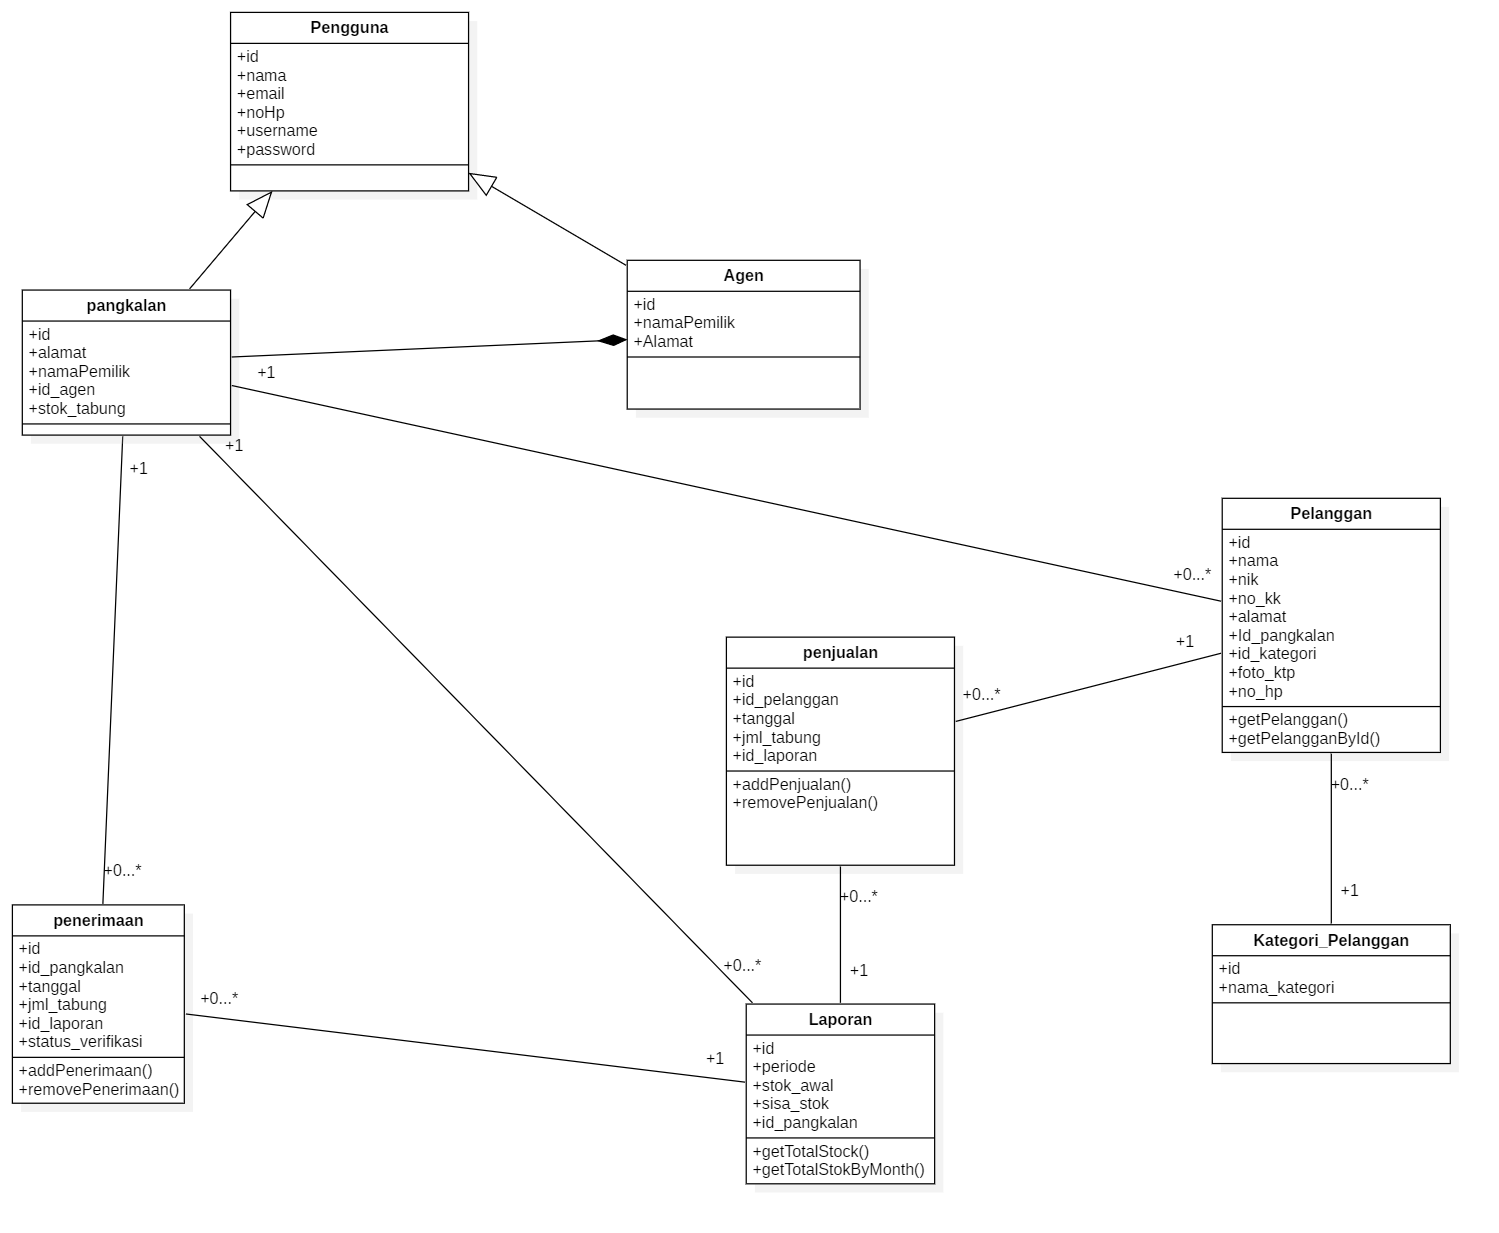
\includegraphics [angle=90,origin=c, width = 17cm]{gambar/model/class-diagram}
\end{figure}

